\documentclass[UTF8]{ctexart}
\usepackage[T1]{fontenc}
\usepackage{makeidx}
\usepackage{tikz}

\usepackage{graphicx} 
\usepackage{float} 
\usepackage{subfigure} 
\usepackage{booktabs}
\usepackage{amsmath}
\usepackage{pgf-pie}
\usepackage{multirow}
\usepackage{pdfpages}
\usepackage[framed,numbered]{matlab-prettifier}
\usepackage{appendix}

\renewcommand\thepage{\zihao{-4} ~\arabic{page}~}
\makeindex
\bibliographystyle{plain}


\begin{document}
\begin{titlepage}
    \centering

    %------------------------------------------------------------
    %    Top rules
    %------------------------------------------------------------

    \rule{\textwidth}{1pt}   % The top horizontal rule

    \vspace{0.2\textheight}  % Whitespace between top horizontal rule and title

    \begin{figure}[H]
        \centering
        \includegraphics[width=0.2\textwidth]{./picture/Xihua_University_logo.png}
    \end{figure}
    %------------------------------------------------------------
    %    Title
    %------------------------------------------------------------
    \begin{center}
		\quad \\
		\quad \\
		\heiti \fontsize{45}{17} 研究报告
		\vskip 3.5cm
		\heiti \zihao{2}  基于TOPSIS环境评价及$PM_{2.5}$含量LSTM神经网络预测
	\end{center}
	% \vskip 3.5cm


    % \vspace{0.025\textheight}   % Whitespace between the title and short horizontal rule

    % \rule{0.83\textwidth}{0.4pt}  % The short horizontal rule under title

    % \vspace{0.1\textheight}  % Whitespace between the short horizontal rule and author

    % %------------------------------------------------------------
    % %    Author
    % %------------------------------------------------------------

    
    % \vfill  % Whitespace between author and date

    % \begin{tikzpicture}
    %    \draw (0,0) sin (1,1) cos (2,0);
    %     \draw (2,0) sin (3,-1) cos (4,0);
    % \end{tikzpicture}
    
    \vfill  % Whitespace between author and date

    {\large \today}
    \vspace{0.1\textheight}  % Whitespace between date and bottom horizontal rule

    %------------------------------------------------------------
    %    Bottom rules
    %------------------------------------------------------------

    \rule{\textwidth}{1pt}  % The bottom horizontal rule

  \end{titlepage}

\newpage


\begin{abstract}
    随着“绿水青山就是金山银山”战略以及“碳达峰和碳中和”目标的提出,表明中国将以新发展理念为引领,在推动高质量发展中促进经济社会全面绿色转型开启绿色低碳时代。
近来环境监测设备已经不是问题,而如何对检测数据进行良好的挖掘成为了有效治理环境污染的重要环节。为了研究环境的发展趋势,首先必须对环境质量做出科学的评价,预测
其发展趋势,科学评价和预测对于实现环境后续保护措施有重要意义。

本文的主要研究内容和创新点如下:


(1)由于环境质量的评价具有主观性,本文从环境评价模型的普适性推广性出发,利用熵权法解决了传统评价模型各评价指标权重一致、无区分度的问题,并结合TOPSIS综合评价模型在很大程度上改进了传统评价方法对指标和数据量要求严苛的局限性。以塞罕坝三十年来的数据为例,可视化地展示了当地环境质量的客观发展趋势。

(2)本文分析了全国各省份的各种空气指标,并利用热力图将全国各省的环境质量进行可视化。分析结果直观,与实际各省份实际空气质量情况相一致。能为环保部门的后续措施提供参考。

(3)本文利用LSTM神经网络对北京市朝阳区从2015年7月17日中午12点至2022年4月12日中午12点每个小时的$PM_{2.5}$的含量,共计50764条$PM_{2.5}$的数据,对接下来一周每小时的空气质量进行预测。

\textbf{关键字:}环境评价 空气质量预测 TOPSIS综合评价模型 LSTM神经网络
\end{abstract}

\newpage
\tableofcontents
\newpage
\section{问题描述与解决办法}
2020年9月,习近平总书记提出“中国二氧化碳排放力争于2030年前达到峰值,努力争取2060年前实现碳中和”的发展目标,自然环境、大气环境越来越受到人们的关注。近年来,国内已经出现了许多环境空气质量实时自动检测系统和重点大气污染源的检测系统。

获取监测数据的系统工程已经日趋完善,现代城市环境空气质量管理面临的主要问题是如何有效管理数据资源并挖掘出数据中蕴含的丰富信息,充分发挥信息潜力及价值$^{[1]}$。基于数据信息的挖掘可以为大气环境的评价以及后续的环境指标预测打下坚实的基础。

% 目前有大量学者提出了关于环境评价和大气污染物、排放物的预测方法。较为主流的评价方法有模糊评价方法;较为主流的预测方法是灰色预测、回归预测和神经网络预测。文献$^{[2]}$提出了模糊评价法在环境评价中的应用,由于环境系统的复杂性,模糊理论的提出有助于降低这种复杂性,模糊理论隶属度的提出很好的降低了指标在系统中的模糊性。文献$^{[3]}$提出一种PLSR回归预测模型,可集成多元线性回归分析,相关性分析和主成分分析,可以很好的解决变量之间存在着多重相关性或样本点过少的回归难题。文献$^{[4]}$也提出利用主成分分析法进行数据降维后的最小二乘回归法,提升了预测精度。文献$^{[5]}$提出了基于灰色系统理论的GM(1,1)预测模型能够挖掘较少数据的发展规律,具有较好的适应性和灵活性。文献$^{[6]}$提出了人工神经网络大气环境数据预测中的应用,人工神经网络具有良好的非线性映射逼近性能,能够充分挖掘大量数据发展规律做出预测。

% 本文的开发是在大气环境监测系统以及完备的数据统计传输系统已经完备的基础上提出的,目前收集数据的系统已经日趋完备,对于所收集数据进行挖掘,环境的评价,大气指标数据预测的系统还不够完备。为了能够充分利用环境监测系统建立起来的历年监测数据,分析大气环境的变化趋势、对空气质量进行预报,目前有学者对此方面做了一些研究,引进了诸如模糊评价、灰色预测、回归预测、神经网络等对大气数据进行评价预测的方法。对比分析以上学者的研究,总结如下关于各模型的优缺点分析:

针对目前研究的局限性,同时为了建立一个具有普适性的环境评价预测系统,引入了熵权法定权模型。可以消除模糊评价、TOPSIS综合评价法各个权重重要性无区分度的局限性。熵权法$^{[7]}$利用熵值来判断某个指标的离散程度,其信息熵值越小,指标的离散程度越大,该指标对综合评价的影响越大,相应的该指标的权重越大。TOPSIS综合评价法$^{[8]}$避免了数据的主观性,不需要目标函数,能够很好的刻画多个影响指标的影响程度;同时TOPSIS综合评价法对数据分布量、指标多少无限制,适用于大样本也适用于小样本,可以适用于多评价单元、多指标的大系统。同时由于TOPSIS模型的普适性,也可以用于其他自然环境指标系统的评价。

目前用于大数据预测时间序列的算法有很多种,诸如AR、MA、ARMA\\模型等。本文使用的数据集高达五万多,数据量很大,一般用于时序分析的都是小样本算法,不适合进行大数据时间序列预测。而长短期记忆神经网络作为循环神经网络的变种,能够比一般的循环神经网络和其他种类的神经网络在更长的时间序列中有更好的表现。


% \begin{figure}[H] %H为当前位置,!htb为忽略美学标准,htbp为浮动图形
%     \centering %图片居中
%     \includegraphics[width=1\textwidth]{./picture/youquedian.png} %插入图片,[]中设置图片大小,{}中是图片文件名
%     \caption{各模型优缺点分析} 
% \end{figure}
\begin{table}[htbp]
    \centering
    \caption{Advantages and disadvantages}
    \begin{tabular}{lll}
    \toprule
    模型 & 优点 & 缺点 \\
    \midrule
    模糊综合评价 & 1.精确的数字手段处& 1.计算复杂,对指标权\\
                & 理模糊的评价对象对& 重矢量的确定主观性较\\
                & 信息呈现模糊性数据& 强。\\
                & 作出比较科学的量化& 2.指标集个数较大时,会\\
                & 评价             & 出现超模糊现象。\\
                & 2.评价结果是一个矢 \\
                & 量,包含的信息比较\\
                & 丰富,可比较准确的\\
                & 刻画被评价对象。\\
    RNN神经网络  & 具有良好的非线性    &1.在处理长序列时经常\\
                & 衍射逼近性能,循环  & 出现“梯度消失“。\\
                & 传递神经网络的数据  &2.隐藏层结构难以确定\\
                & 具有一定的记忆力。 \\                  
    LSTM神经网络 & 可以拟合序列数据   & 1.LSTM虽然部分解决了\\
                &(LSTM)通过遗忘门   & rnn梯度消失问题,但\\ 
                & 和输出门忘记部分信 & 是信息在过远的距离传\\
                & 息来解决梯度消失的 & 播中损失很厉害 \\
                & 问题。            & 2.无法很好的并行 \\
    \bottomrule
    \end{tabular}
    \label{table1}
\end{table}

表\ref{table1}是本文使用的算法的优缺点。


\newpage
\section{模型适用性检验}
\subsection{数据来源}
本文所有的数据均来自国家统计局、河北省统计局和开源空气质量组织(OpenAQ)的网站。

\subsection{数据分析和处理}
由于塞罕坝在过去的几十年间环境改造取得了举世瞩目的成果,本文通过选取塞罕坝环境数据来检验模型的适用性,通过查询国家统计局数据库得到河北市塞罕坝森林覆盖率、森林覆盖面积、林木蓄积、涵养水量、二氧化碳吸收量、氧气释放量6个环境评价指标自1962年至2021年间的完整数据。
首先对获取的塞罕坝数据利用SPSS软件进行描述统计:

\begin{figure}[H] %H为当前位置,!htb为忽略美学标准,htbp为浮动图形
    \centering %图片居中
    \includegraphics[width=0.7\textwidth]{./picture/datascrip.png} %插入图片,[]中设置图片大小,{}中是图片文件名
    \caption{数据描述统计图} 
\end{figure}


变异系数CV:
\begin{equation}
    CV=\frac{\delta}{\mu}
\end{equation}

其中为样本数据的标准差, 为样本数据的平均值.

当需要比较数据离散程度大小的时候,如果数据的测量尺度相差太大,或者数据量纲的不同,直接使用标准差来进行比较不合适,此时就应当消除测量尺度和量纲的影响,而变异系数可以做到这一点,标准差与其平均数的比。CV虽然没有量纲,同时又按照其均数大小进行了标准化,这样就可以进行客观比较了。因此,可以认为变异系数和极差、标准差和方差一样,都是反映数据离散程度的绝对值。其数据大小不仅受变量值离散程度的影响,而且还受变量值平均水平大小的影响。
\begin{figure}[H] %H为当前位置,!htb为忽略美学标准,htbp为浮动图形
    \centering %图片居中
    \includegraphics[width=1\textwidth]{./picture/biaoge1.png} %插入图片,[]中设置图片大小,{}中是图片文件名
    \caption{变异系数} 
\end{figure}

当变异系数CV>0.15时,可认为数据中有异常值:

\begin{enumerate}
\item 基于二氧化碳吸收量/万吨,变异系数(CV)为0.875,大于0.15,当前数据中可能存在异常值,建议对异常的或者表现得较为突出的指标进行分析。
\item 基于森林覆盖率,变异系数(CV)为0.344,大于0.15,当前数据中可能存在异常值,建议对异常的或者表现得较为突出的指标进行分析。
\item 基于氧气释放量/万吨,变异系数(CV)为0.875,大于0.15,当前数据中可能存在异常值,建议对异常的或者表现得较为突出的指标进行分析。
\item 基于涵养水量/亿立方米,变异系数(CV)为0.956,大于0.15,当前数据中可能存在异常值,建议对异常的或者表现得较为突出的指标进行分析。
\item 基于覆盖面积/万亩,变异系数(CV)为0.344,大于0.15,当前数据中可能存在异常值,建议对异常的或者表现得较为突出的指标进行分析。
\item 基于林木蓄积/万立方米,变异系数(CV)为0.875,大于0.15,当前数据中可能存在异常值,建议对异常的或者表现得较为突出的指标进行分析。
\end{enumerate}

\subsection{异常值处理}
一组数据只含有随机误差,对其进行计算处理得到标准偏差,按一定概率确定一个区间,认为凡超过这个区间的误差,就不属于随机误差而是粗大误差,含有该误差的数据应予以剔除。这种判别处理原理及方法仅局限于对正态或近似正态分布的样本数据处理,它是以测量次数充分大为前提。根据3 $\sigma$原则。
\begin{equation}
    \text{原则}=\left \{
         \begin{aligned}
            \text{数值分布在(μ-δ,μ+δ)中的概率为0.6826}\\
            \text{数值分布在(μ-2δ,μ+2δ)中的概率为0.9544}\\
            \text{数值分布在(μ-3δ,μ+3δ)中的概率为0.9974}
         \end{aligned}
     \right.
\end{equation}

对样本进行等精度测量,独立得到$x_1,x_2,...,x_n$算出其算术平均值 ,以及剩余误差 ,并计算标准差 ,当样本值 满足:
\begin{equation}
    \left|v_i\right|=\left|x_i-x\right|>3\delta
\end{equation}

则$x_i$应该剔除。据此,筛选出样本中的异常值。对于异常值的处理采用相邻两数据的平均值进行替换。

\begin{figure}[H] %H为当前位置,!htb为忽略美学标准,htbp为浮动图形
    \centering %图片居中
    \includegraphics[width=0.7\textwidth]{./picture/saihanbapj.png} %插入图片,[]中设置图片大小,{}中是图片文件名
    \caption{塞罕坝环境评价指标} 
\end{figure}

建立塞罕坝对生态环境的影响评价模型是对评价方法的应用,目前综合评价方法多种多样,如模糊评价法、加权平均法、层次分析法、主成分分析法、熵权评价法、灰色关联评价法、TOPSIS方法和数据包络法等。本文结合熵权法和TOPSIS方法,分析塞罕坝地区改造对环境影响问题。

\newpage
\section{综合评价方法介绍}
\subsection{熵权法}
熵权法是一个客观的赋权方法,可以最大程度上避免主观性赋权对于环境指标量化结果的影响。熵权法权法依据的原理是指标的变异程度,即变异程度越高则对应的权值也就越高。

首先本文需要对环境指标数据进行正向化和归一化处理,保证数据的统一性:
\begin{equation}
    z_{ij}=\frac{x_{ij}-x_{min}}{{xmax}_{max}}
\end{equation}

其中 为归一化处理后的变量,$x_{min}$和 $x_{max}$分别为每个指标的最大值和最值。
计算第j个环境指标下第i个年份所占权重,将其看作计算信息熵时的概率 
\begin{equation}
    p_{ij}=\frac{z_{ij}}{\sum_{i=1}^{n}z_{ij}} 
\end{equation}

计算第j个环境指标的信息熵 ,并计算对应信息效用值 ,此处进行转换的原因是因为信息熵越大代表该环境指标的信息越少,引入 就可以正向衡量信息量。
\begin{equation}
    e_j=-\frac{1}{ln{n}}\sum_{i=1}^{n}{ln{(}p_{ij})}
\end{equation}
\begin{equation}
    d_j=1-e_j
\end{equation}

最终归一化得到每个环境评价指标的熵权$w_j$
\begin{equation}
    w_j=\frac{d_j}{\sum_{j=1}^{m}d_j}
\end{equation}

得到6个权重分别为:

\begin{table}[H]
    \begin{tabular}{lllll}
        \hline
        \multicolumn{1}{|l|}{}        & \multicolumn{1}{l|}{森林覆盖率}   & \multicolumn{1}{l|}{森林覆盖面积} & \multicolumn{1}{l|}{林木面积}   & \multicolumn{1}{l|}{涵养水量}   \\ \hline
        \multicolumn{1}{|l|}{Weights} & \multicolumn{1}{l|}{0.0561}  & \multicolumn{1}{l|}{0.0561} & \multicolumn{1}{l|}{0.2198} & \multicolumn{1}{l|}{0.2309} \\ \hline
                                      &                              &                             &                             &                             \\ \cline{1-3}
        \multicolumn{1}{|l|}{}        & \multicolumn{1}{l|}{二氧化碳吸收量} & \multicolumn{1}{l|}{氧气释放量}  &                             &                             \\ \cline{1-3}
        \multicolumn{1}{|l|}{Weights} & \multicolumn{1}{l|}{0.2198}  & \multicolumn{1}{l|}{0.2198} &                             &                             \\ \cline{1-3}
        \end{tabular}
    \caption{权重表}
\end{table}



塞罕坝环境综合评价一项较为复杂的系统工程,在研究此问题时不能忽视指标本身所蕴含的信息。采用了熵权分析法来处理指标权重。按照信息论最基本的原理,信息作为系统有序程度的度量,熵则是系统无序程度的度量,熵权法利用熵值来判断某个指标的离散程度,其信息熵值越小,指标的离散程度越大,该指标对综合评价的影响越大,相应的该指标的权重越大。 
\subsection{TOPSIS综合评价法}
TOPSIS法是用来处理指标决策问题的多方案排序和选择的方法,它的基本思想是:依据理想点的理论原理,找寻距离理想点最近的方案。并通过计算对象与最优解、最劣解的距离大小,确定顺序。即先设定一个虚拟的最优解(又称正理想解)和一个最劣解(又称负理想解),将各备选方案与正负理想解相互比较,若方案最靠近最优解即又距最劣解最远为最好。另外,TOPSIS方法需要的评价指标决策矩阵和指标权重,由上文中的熵权法计算给出。

所选指标均为效益性指标,故不做另外处理。找出每列也就是每个环境指标的最大值,记为$z_i^+(i=1,2,...,m)$ ,组成向量
\begin{equation}
    Z^+={z_1^+,z_2^+,...,z_m^+}
\end{equation}

该向量代表了环境最好的年份。同样的,找出每列也就是每个指标的最小值,记为$z_i^-(i=1,2,...,m)$ ,组成向量

\begin{equation}
    Z^-={z_1^-,z_2^-,...,z_m^-}
\end{equation}

该向量代表了环境最差的年份。

定义第i个年份与理想目标距离为$D_i^+$ ,计算公式为
\begin{equation}
    D_i^+=\sqrt{\sum_{j=1}^{m}{w_j(z_j^+-z_{ij})^2}}
\end{equation}

定义第i个年份与不理想目标距离为$D_{ij}^-$,计算公式为
\begin{equation}
    D_i^+=\sqrt{\sum_{j=1}^{m}{w_j(z_j^+-z_{ij})^2}}
\end{equation}

定义第i个年份的得分为$S_i$,计算公式为
\begin{equation}
    S_i=\frac{D_i^-}{D_i^++D_i^-}
\end{equation}
显然,$S_i\in[0,1]$当$S_i$越接近于1,说明此年份i距离理想化目标越近,该年份塞罕坝环境就越好。反之,当 越接近于0,说明年份i距离理想化目标越远,该年份塞罕坝环境就越差。

计算数据得到1962-2021年间塞罕坝环境的量化得分:

\begin{figure}[H] %H为当前位置,!htb为忽略美学标准,htbp为浮动图形
    \centering %图片居中
    \includegraphics[width=0.7\textwidth]{saihanba.png} %插入图片,[]中设置图片大小,{}中是图片文件名
    \caption{塞罕坝评价历年环境指数} 
\end{figure}

根据评价模型得出的1962年到2021年塞罕坝环境得分呈上升趋势,可知塞罕坝恢复对环境改造有积极作用。塞罕坝几代人的防沙治沙卓有成效,不仅留下了巨大精神财富,也为后来环境改造工程提供了范本。

\newpage
\section{大气环境综合评价}
目前全国的环境保护监测站已经建立起一套十分完备的城市环境质量监测系统,包括空气质量实时监测系统和重点污染源在线监控系,使得全国各地的空气质量监测数据都能通过系统上传到城市环境空气质量数据库$^{[9]}$最终被国家统计局收录,本文从国家统计局官网下载2021年12月各个市份$PM_{2.5}$、$PM_{10}$、AQI(空气质量指数)作为评价指标数据来研究本文中模型的适用性。

\subsection{$PM_{2.5}$浓度和$PM_{10}$}
大气污染物因子有很多种,当前我国环境保护部门监测环境空气污染物时采用的是$PM_{10}$这个指标。其定义是空气中当量直径为10μm的尘埃或飘尘的浓度。由此,可知$PM_{2.5}$是直径小于或等于2.5μm的尘埃或飘尘在环境空气中的浓度$PM_{2.5}$。$PM_{2.5}$和$PM_{10}$的主要成分包括:含碳颗粒(包括元素碳和有机碳,元素碳主要产生于高温燃烧过程,有机碳则主要来自相对低温过程的不完全燃烧产物)、硫酸盐、硝酸盐、铵盐、重金属等。$PM_{2.5}$和$PM_{10}$在空气悬浮过程中还会进一步吸附空气中存在的有机和金属等化学成分、细菌、病毒、真菌等微生物成分。对空气质量破坏明显,对人体危害极大。

\subsection{AQI(空气质量指数)}
空气质量指数(Air Quality Index,简称AQI),是一个用来定量描述空气质量水平的数值。AQI的取值范围位于0-500 之间。环境空气污染物的种类有很多,参与AQI指数评价的有二氧化硫(SO2)、二氧化氮(NO2)、一氧化碳(CO)、臭氧(O3)、$PM_{2.5}$、$PM_{10}$。

\begin{figure}[H] %H为当前位置,!htb为忽略美学标准,htbp为浮动图形
    \centering %图片居中
    \includegraphics[width=0.7\textwidth]{./picture/AQI.png} %插入图片,[]中设置图片大小,{}中是图片文件名
    \caption{AQI评价指标内容} 
\end{figure}

环境监测部门每天发布的空气质量报告中,会包含各种污染物的浓度值。很难从这么多个抽象的浓度数据中判断出到底当前的空气质量处在什么水平。于是将各种不同污染物含量折算成一个统一的指数,这就是空气质量指数。 空气质量指数的值在不同的区间,就代表了不同的空气质量水平。比如0-50之间,代表良好;51-100之间,代表中等;101-150之间代表轻度污染等等。为了更直观起见,每个区间都有一个固定的颜色值与它对应:

\begin{figure}[H] %H为当前位置,!htb为忽略美学标准,htbp为浮动图形
    \centering %图片居中
    \includegraphics[width=0.9\textwidth]{./picture/biaoge2.png} %插入图片,[]中设置图片大小,{}中是图片文件名
    \caption{AQI数据对应表} 
\end{figure}

AQI的折算公式如下:
\begin{equation}
    I=\frac{I_{high}-I_{low}}{C_{high}-C_{low}}(C-C_{low})+I_{low}
\end{equation}

其中I等于空气质量指数,即AQI,输出值;C为污染物浓度,输入值;$C_{low}$为小于或等于C的浓度限值$C_{high}$为大于或等于C的浓度限值;$I_{low}$对应于$C_{low}$的指数限值;$I_{high}$为对应于$C_{high}$的指数限值。将计算好的数据按照从低到高进行排序并使用matlab绘制出条形图。

\begin{figure}[H] %H为当前位置,!htb为忽略美学标准,htbp为浮动图形
    \centering %图片居中
    \includegraphics[width=0.9\textwidth]{./picture/geshengpaiming.png} %插入图片,[]中设置图片大小,{}中是图片文件名
    \caption{各省环境质量排名图} 
\end{figure}

\newpage
利用Matlab编程得到环境质量指数热力图,将各个省份的数据可视化后,可以看出我国南方地区普遍空气质量较好。
除开新疆沙漠的原因导致的气候异常,华北平原和华中平原目前属于环境空气污染较为严重的地区。

\begin{figure}[H] %H为当前位置,!htb为忽略美学标准,htbp为浮动图形
    \includegraphics[width=1\textwidth]{./picture/ChinaMap.pdf} %插入图片,[]中设置图片大小,{}中是图片文件名
    \caption{全国环境质量指数热力图} 
\end{figure}

\newpage
\section{空气质量变化预测分析}
为了预测北京市朝阳区后续的空气质量变化,本文使用了China - OpenAQ组织的Beijing US Embassy项目中北京市朝阳区2015年7月17日中午12点-2022年4月12日中午十二点每个小时的$PM_{2.5}$含量,共50764条数据,清洗后的数据如下图所示。
\begin{figure}[H] %H为当前位置,!htb为忽略美学标准,htbp为浮动图形
    \centering %图片居中
    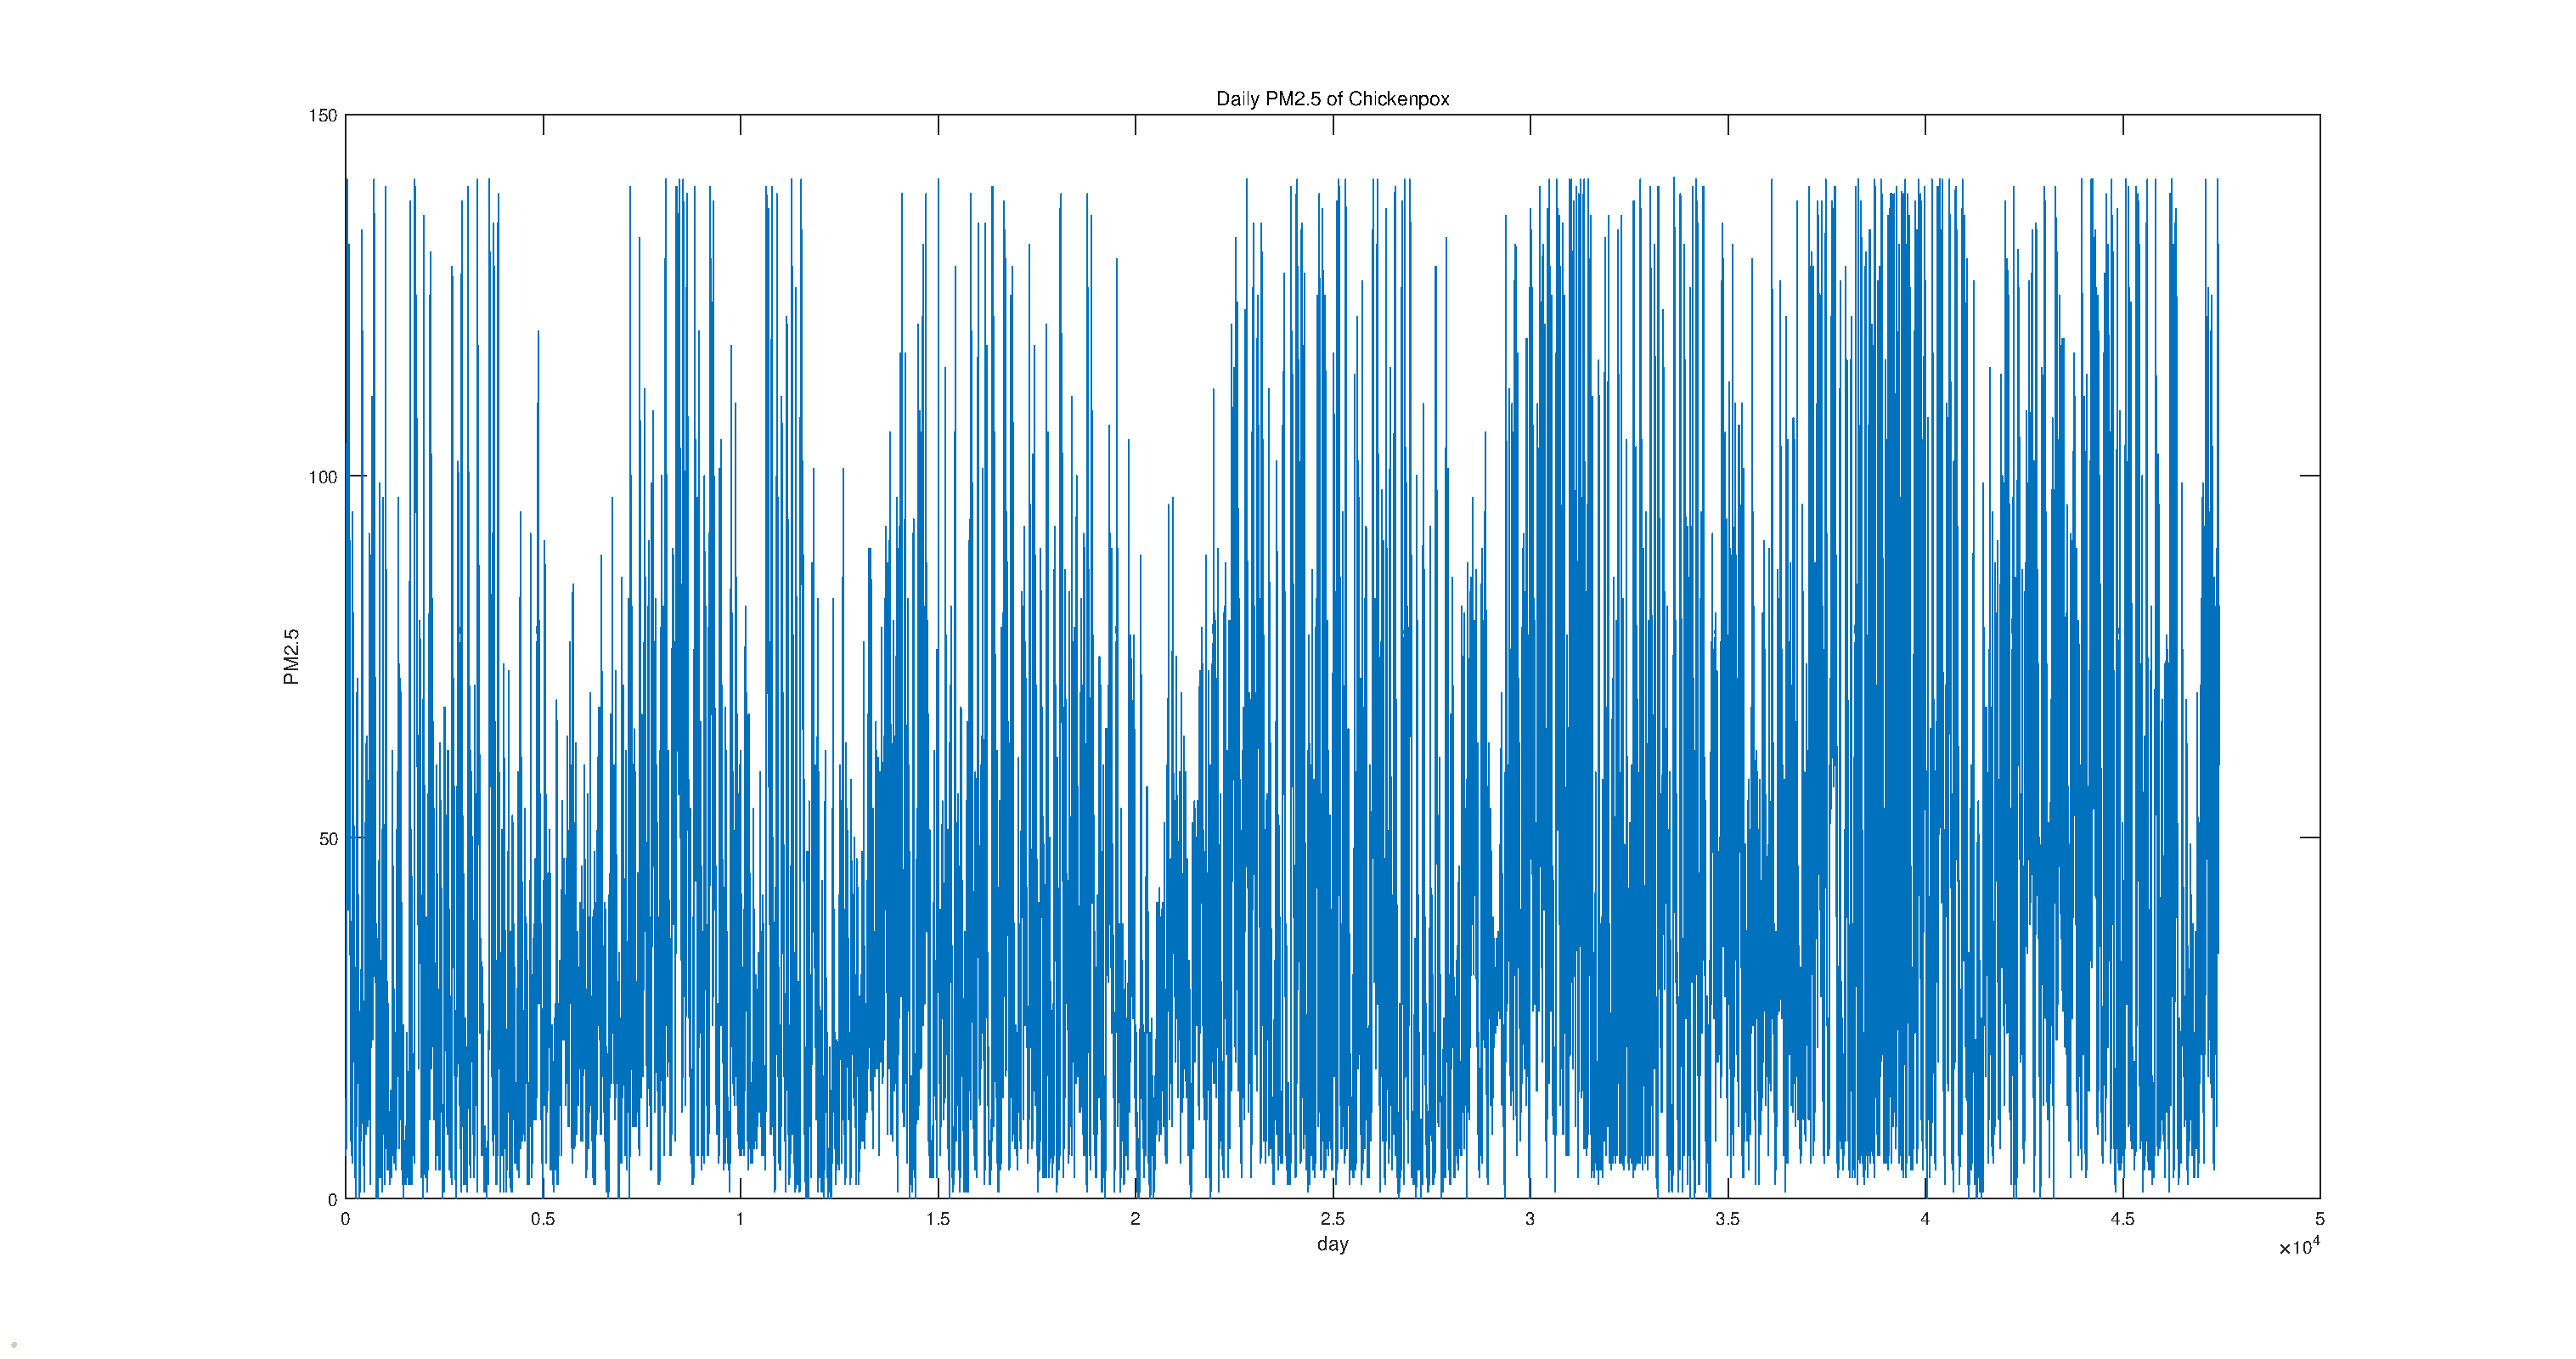
\includegraphics[width=0.9\textwidth]{./picture/DailyPM2.5ofhickenpoxeps.eps} %插入图片,[]中设置图片大小,{}中是图片文件名
    \caption{清洗后$PM_{2.5}$分布图} 
\end{figure}

将清洗后的数据使用中国气象局的标准$^{[4]}$转换为空气质量指标,北京市朝阳区近2115天中的优的空气质量占52\%,良占\%29,轻度污染占10\%,中度污染占4\%,重度污染占1\%,严重污染占1\%。
\begin{figure}[H]
    \centering
    \begin{tikzpicture}
         \pie[text=legend,explode={0.1,0,0,0,0,0},rotate = 90]{52/优,29/良,10/轻度污染,4/中度污染,4/重度污染,1/严重污染}
    \end{tikzpicture}
    \caption{北京市朝阳区空气质量饼图}
\end{figure}

\subsection{RNN神经网络介绍}
处理与事件发生的时间轴有关系的问题时,比如自然语言处理,文本处理,文字的上下文是有一定的关联性的;时间序列数据,如连续几天的天气状况,当日的天气情况与过去的几天有某些联系;又比如语音识别,机器翻译等。在考虑这些和时间轴相关的问题时,传统的神经网络就无能为力了,因此就有了RNN(recurrent neural network,循环神经网络)。

RNN之所以被称为循环神经网络是因为一个序列的输出与前一时刻的输出有关,前面数据信息会影响后一个输出,隐含层的节点是相互关联的。

RNN网络结构如下图所示,RNN模型结构展开图见图l,其中α表示输入样本,y表示训练后的输出样本,t-1,t,t+1分别表示时间序列,U、W、V是在每一刻都共享的网络权重,U为某一时刻输入样本的权重、W为隐含层的权重、V表示输出的样本权重。 表示当前t 时刻的隐藏状态,由当前时刻的输入样本x,和t-1时刻的隐藏状态共同决定,表达式为:
\begin{equation}
    s_i=f(Ux_i+W_{S_t-1})
\end{equation}
\begin{equation}
    y_i=g(V_{S_I})
\end{equation}

\begin{figure}[H] %H为当前位置,!htb为忽略美学标准,htbp为浮动图形
    \centering %图片居中
    \includegraphics[width=0.9\textwidth]{./picture/RNMNetStructural.png} %插入图片,[]中设置图片大小,{}中是图片文件名
    \caption{RNN网络结构图} 
\end{figure}
\subsection{LSTM神经网络介绍}
长短期记忆(Long short-term memory, LSTM)是一种改进的RNN,主要是为了解决长序列训练过程中的梯度消失和梯度爆炸问题。长短期记忆网络的结构如下图所示,在一般的循环神经网络中,记忆单元没有衡量信息的价值量的能力,因此,记忆单元对于每个时刻的状态信息等同视之,这就导致了记忆单元中往往存储了一些无用的信息,而真正有用的信息却被这些无用的信息弱化。LSTM正是从这一点出发做了相应改进,和一般结构的循环神经网络只有一种网络状态不同,LSTM中将网络的状态分为内部状态和外部状态两种。LSTM的外部状态类似于一般结构的循环神经网络中的状态,即该状态既是当前时刻隐藏层的输出,也是下一时刻隐藏层的输入。这里的内部状态则是LSTM特有的。   
\begin{figure}[H] %H为当前位置,!htb为忽略美学标准,htbp为浮动图形
    \centering %图片居中
    \includegraphics[width=0.9\textwidth]{./picture/LSTMNetStructural.png} %插入图片,[]中设置图片大小,{}中是图片文件名
    \caption{RNN网络结构图} 
\end{figure}

在LSTM中有三个称之为“门”的控制单元,分别是输入门(input gate)、输出门(output gate)和遗忘门(forget gate),其中输入门和遗忘门是LSTM能够记忆长期依赖的关键。输入门决定了当前时刻网络的状态有多少信息需要保存到内部状态中,而遗忘门则决定了过去的状态信息有多少需要丢弃。最后,由输出门决定当前时刻的内部状态有多少信息需要输出给外部状态。
遗忘门:
\begin{equation}
    n_t=\delta(W_n[ht-1,xt]+bn)
\end{equation}

输入门:
\begin{equation}
    l_t=\delta(W_l[ht-1,xt]+bi)
\end{equation}
\begin{equation}
    r_t=tanh{(}W_r[ht-1,xt]+br)
\end{equation}
\begin{equation}
    c_t=n_t\ast c_{t-1}+l_t*r_t
\end{equation}

输出门:
\begin{equation}
    m_t=\delta(W_m[hi-1,xt]+bm)
\end{equation}
\begin{equation}
    h_t=m_t*tanh{(}c_t)
\end{equation}
其中 为sigmoid激活函数将数据映射到0-1之间:
\begin{equation}
    f(x)=\frac{1}{1+e^{-x}}
\end{equation}

tanh是双曲正切激活函数, 表示当前时刻的样本输人,其中, 为权值矩阵, 表示为参数矩阵,  表示遗忘门输出,  为输入门输入,  为输出门输出, 表示当前时刻保存的信息。

本文使用两个不同隐藏层结构的LSTM神经网络,分别用于实时预测和72小时预测。

\subsection{模型评价}
模型误差大多采用如下三种公式进行计算。

均方误差(MSE):
\begin{equation}
    MSE=\frac{1}{n}\sum_{i=1}^{n}{(\hat{y}-y)^2}
\end{equation}

平均相对误差(MAE):
\begin{equation}
    MAE=\frac{1}{n}\sum_{i=1}^{n}\left|\hat{y}-y\right|
\end{equation}

根均方误差(RMSE):
\begin{equation}
    RMSE=\sqrt{\frac{1}{n}\sum_{i=1}^{n}{(\hat{y}-y)^2}}
\end{equation}

而本文使用第三种方式进行误差评估,理由是根均方误差度量模型所预测的值与实际值之间的平均差值,表示了相对于真实值的离散程度,根均方误差的值越小,模型的质量越好。
\subsection{数据清洗}
利用Matlab进行LSTM神经网络训练时,首先需要对数据进行清洗。本文将比上四分位数 (75\%) 大 1.5 个四分位差以上或比下四分位数 (25\%) 小 1.5 个四分位差以上的元素和低于0值的元素作为离群值进行删除。将含量低于0微克/立方公尺的元素清除的理由是$PM_{2.5}$的含量不可能低于0。

空缺值使用相邻非缺失值的线性插值。

清洗前数据分布为:
\begin{figure}[H] %H为当前位置,!htb为忽略美学标准,htbp为浮动图形
    \centering %图片居中
    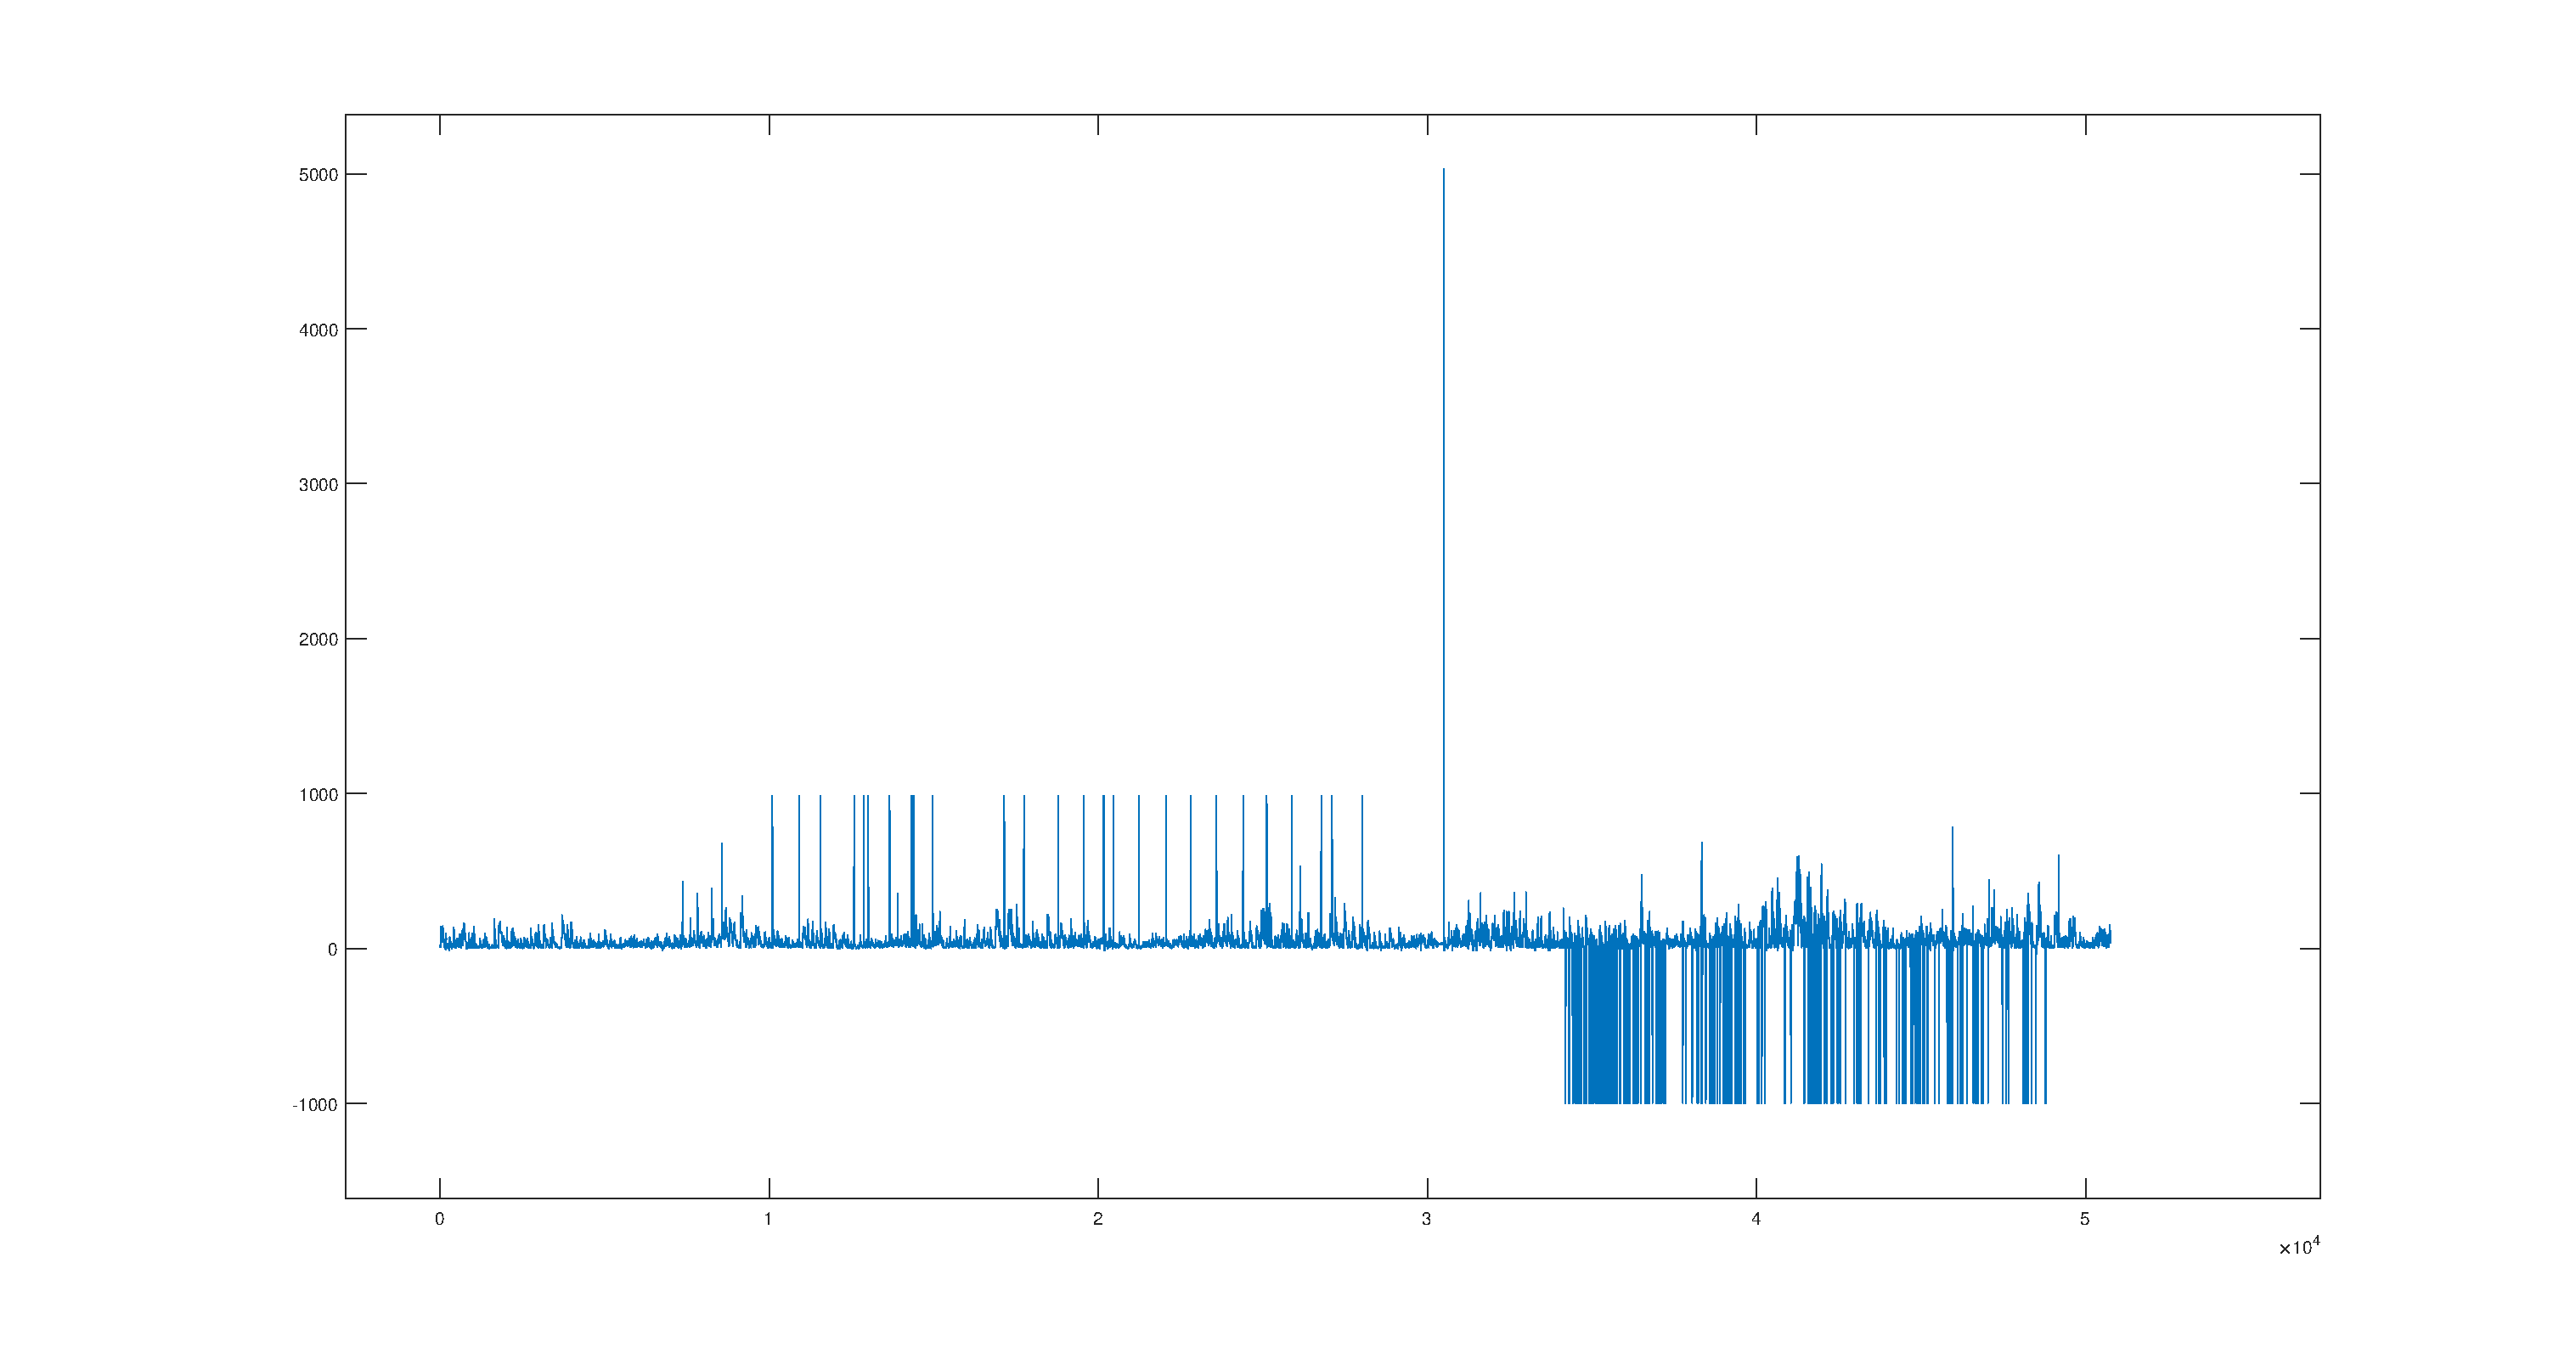
\includegraphics[width=0.9\textwidth]{./picture/untide.eps} %插入图片,[]中设置图片大小,{}中是图片文件名
    \caption{清洗前$PM_{2.5}$分布图} 
\end{figure}

清洗后数据分布为:
\begin{figure}[H] %H为当前位置,!htb为忽略美学标准,htbp为浮动图形
    \centering %图片居中
    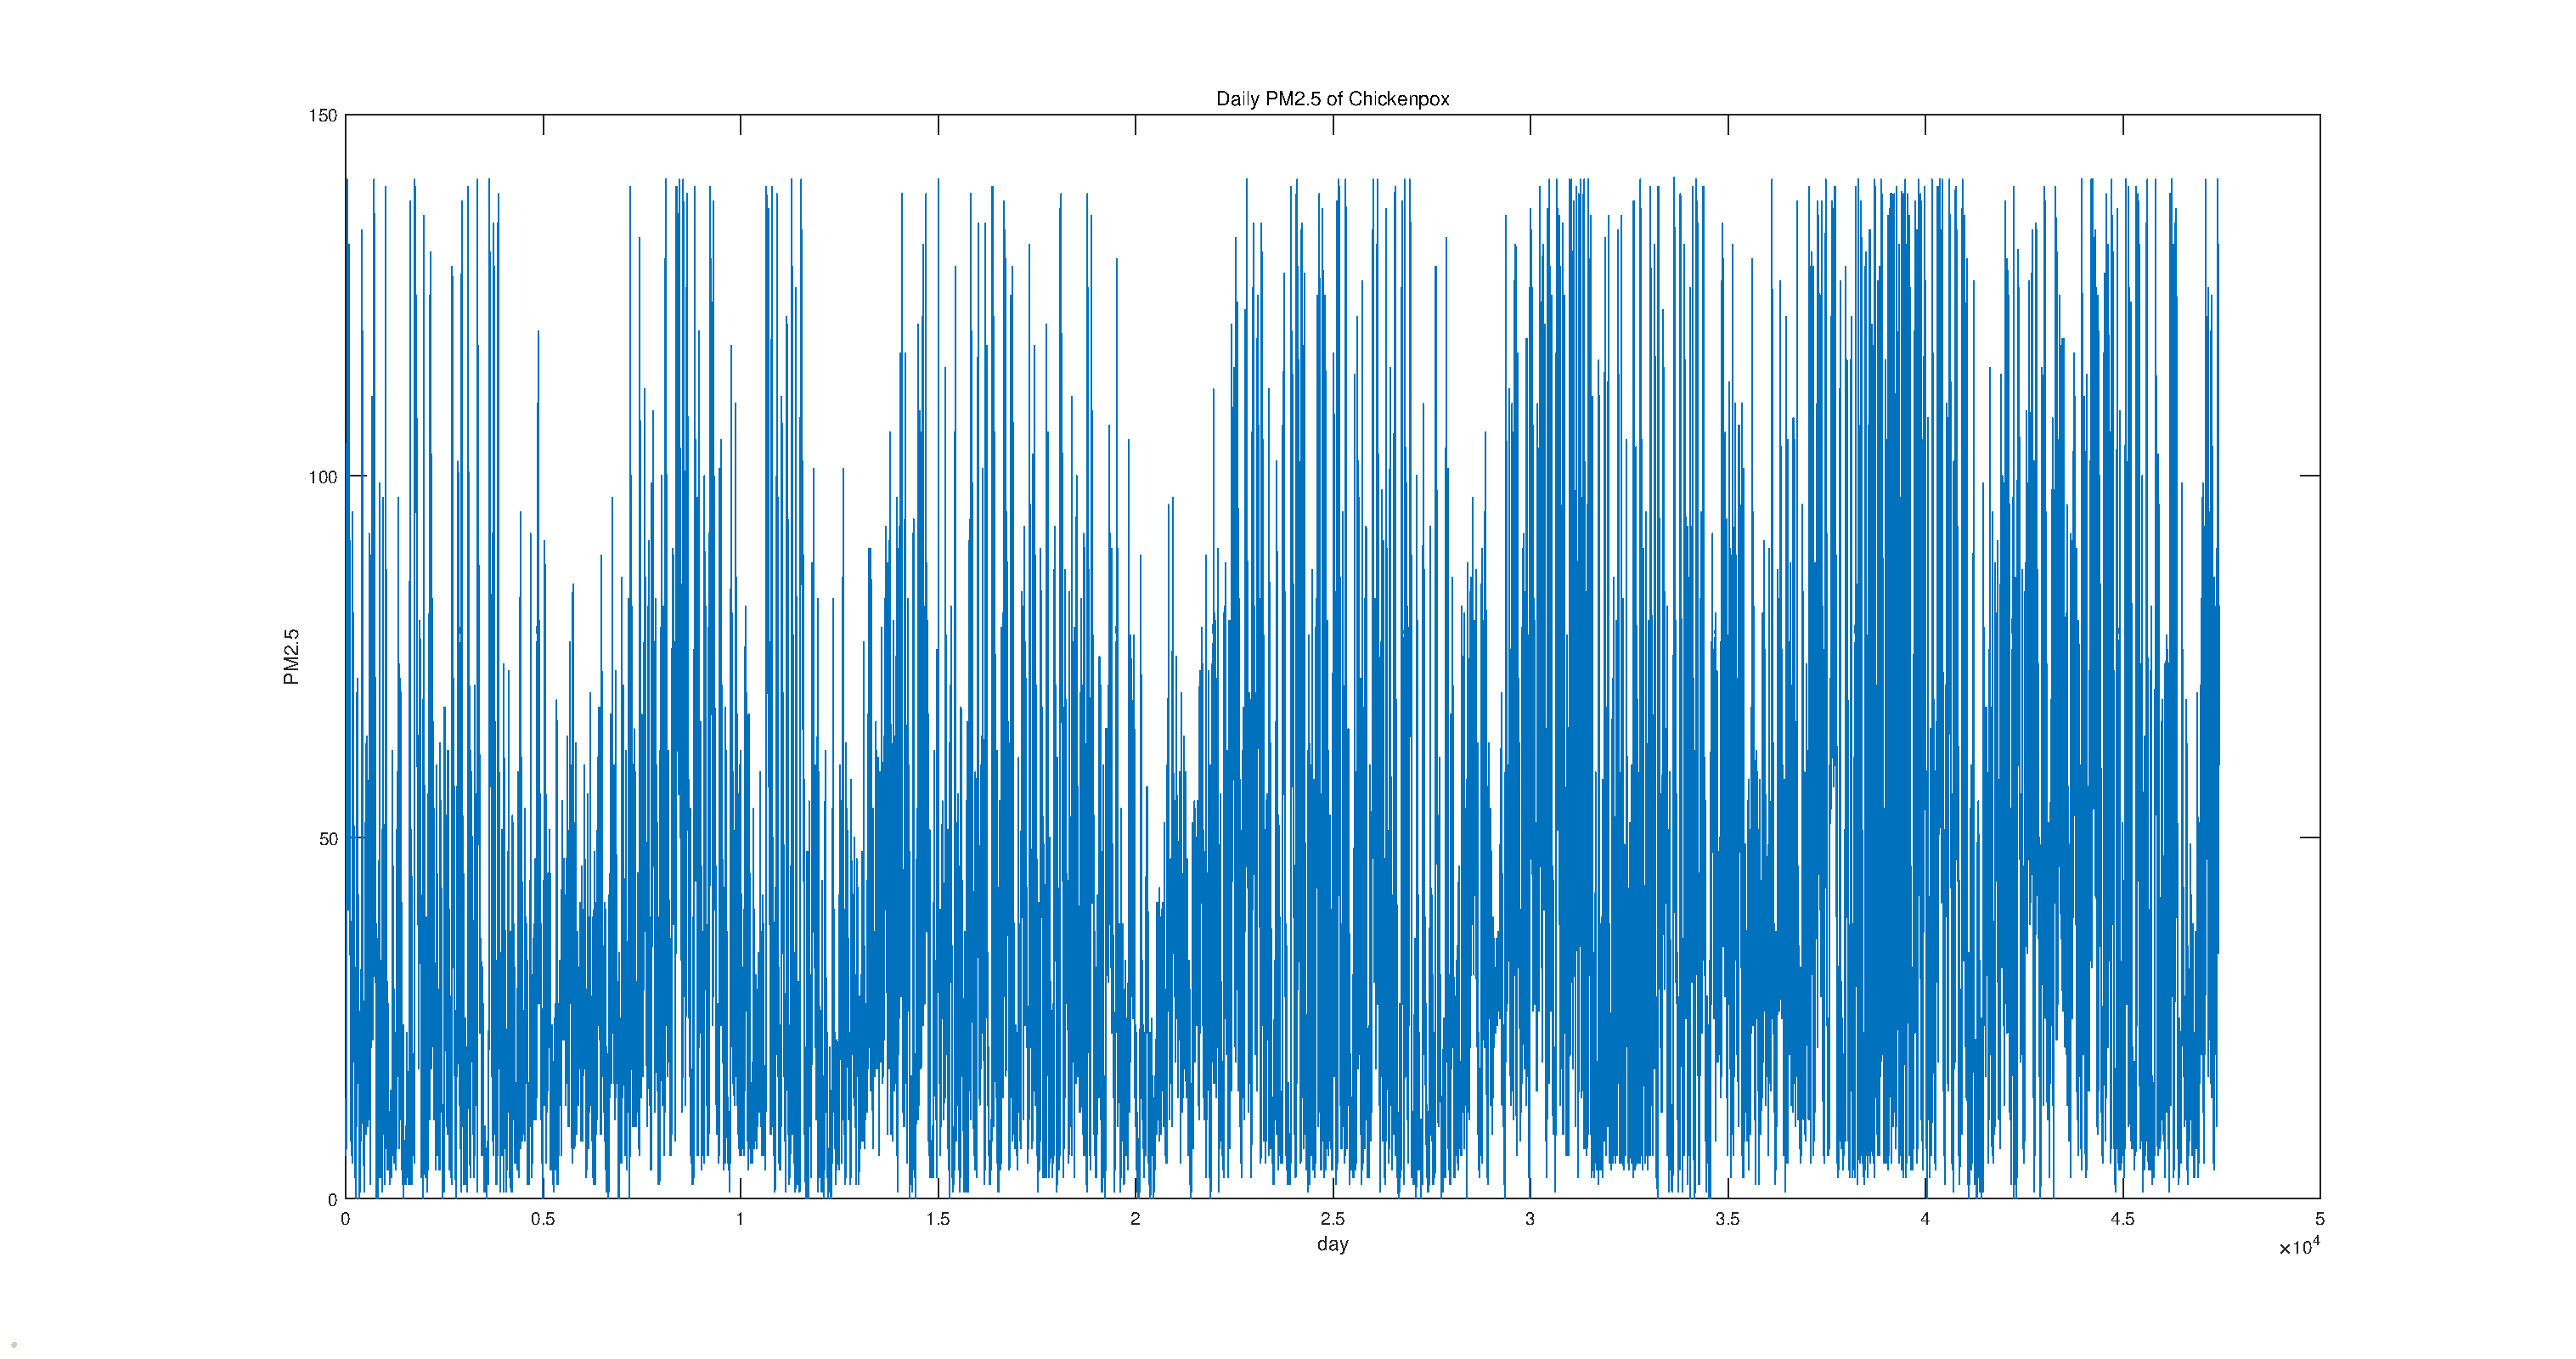
\includegraphics[width=0.9\textwidth]{./picture/DailyPM2.5ofhickenpoxeps.eps} %插入图片,[]中设置图片大小,{}中是图片文件名
    \caption{清洗后$PM_{2.5}$分布图} 
\end{figure}

\newpage
\subsection{LSTM神经网络预测}
\subsubsection{LSTM神经网络实时预测}
本文用于实施预测的LSTM神经网络的网络结构如表\ref{NetStruct1}所示
    \begin{table}[H]
        \centering
        \begin{tabular}{|l|llll|}
            \hline
            \multirow{7}{*}{LSTM} & \multicolumn{4}{l|}{Input Layer(1)}    \\ \cline{2-5} 
                & \multicolumn{4}{l|}{Fully Connected Layer(200)} \\ \cline{2-5} 
                & \multicolumn{4}{l|}{LSTM Layer(200)}            \\ \cline{2-5} 
                & \multicolumn{4}{l|}{Dropout Layaer(0.2)}        \\ \cline{2-5} 
                & \multicolumn{4}{l|}{Fully Connected Layer(200)} \\ \cline{2-5} 
                & \multicolumn{4}{l|}{Fully Connected Layer(1)}   \\ \cline{2-5} 
                & \multicolumn{4}{l|}{Regression Layer}           \\ \hline
        \end{tabular}
        \caption{实时预测LSTM神经网络结构}
        \label{NetStruct1}
    \end{table}
使用的隐藏层为五层,第一层是有200个神经元的全连接层,第二层有200个神经元的LSTM层,第三层抛弃层遗忘率设置为0.2,第四层是有200个神经元的全连接层,第五层是有1个神经元的全连接层用于输出。
前125次的学习率设置为0.0005,后125次的学习率设置为0.25。

\begin{figure}[H] %H为当前位置,!htb为忽略美学标准,htbp为浮动图形
    \centering %图片居中
    \includegraphics[width=0.9\textwidth]{./picture/TrainingProgress1.png} %插入图片,[]中设置图片大小,{}中是图片文件名
    \caption{根均方误差图和损失函数图}
    \label{res1} 
\end{figure}
从图\ref{res1}中可以看到模型在第50次训练后,以后基本上使得根均方差保持在了0.3左右,同时损失值也相对降低到了最低值。前期训练使用0.0005的学习率是为了更精确找到损失函数的最小值,在后面125次训练中使用较大的学习率是为了防止梯度爆炸而陷入局部优解,错过最优解。

处理后的数据有50764条数据,将其前90\%的数据作为训练集,将剩余的10\%的数据作为测试集。设置好神经网络的结构后,使用CPU进行计算并使用实时更新数据集的方式进行预测训练。

训练结束后,将预测数据与测试数据进行对比,计算根均方差,结果如下。
\begin{figure}[H] %H为当前位置,!htb为忽略美学标准,htbp为浮动图形
    \centering %图片居中
    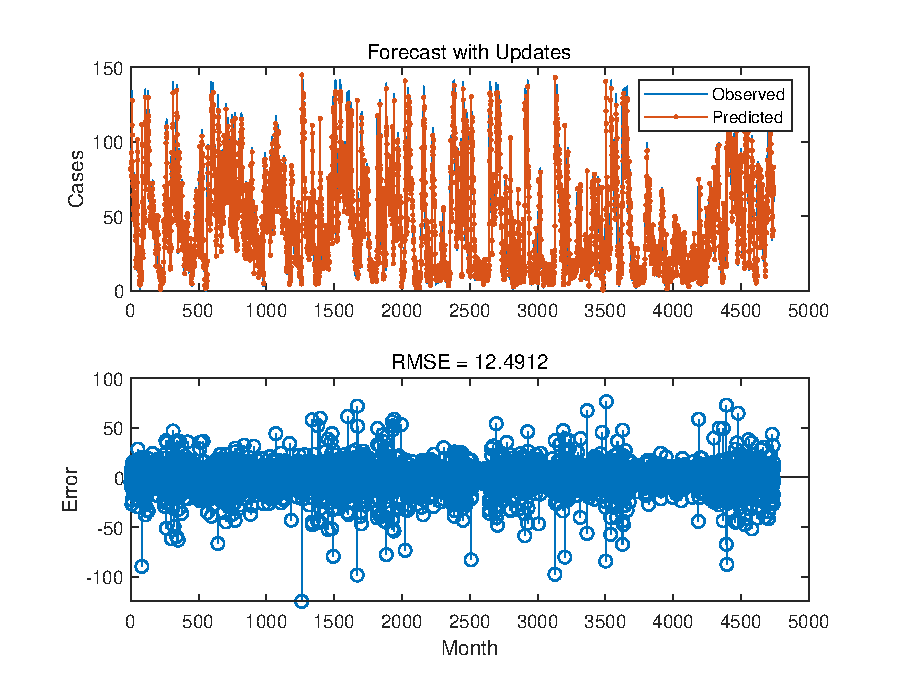
\includegraphics[width=0.7\textwidth]{./picture/ForecasetWithUpdates.eps} %插入图片,[]中设置图片大小,{}中是图片文件名
    \caption{实时预测和根均方误差(RMSE)} 
    \label{LastingPre}
\end{figure}
其中,根均方差为7.409。

考虑到只进行数值上的预测不够直观,于是将预测结果和真实值换算成气象局$^{[4]}$规定的空气质量指标。由于图\ref{LastingPre}中测试数据较多,附录中存取了24小时的预测数据用于参考。
表\ref{hours24}只选取了24小时实时预测的部分数据作为文章内容中的演示,完整的预测表格表\ref{allhours24}可以在附录找到。

\begin{table}[H]
    \centering
    \begin{tabular}{|c|c|clll|}
    \hline
    \multicolumn{1}{|l|}{时间} & \multicolumn{1}{l|}{预测等级} & \multicolumn{4}{l|}{实际等级} \\ \hline
    第1个小时                     & 优                         & \multicolumn{4}{c|}{优}    \\ \hline
    第2个小时                    & 优                         & \multicolumn{4}{c|}{优}    \\ \hline
    ...                     & ...                         & \multicolumn{4}{c|}{...}    \\ \hline
    第23个小时                     & 优                         & \multicolumn{4}{c|}{优}    \\ \hline
    第24个小时                     & 优                         & \multicolumn{4}{c|}{优}    \\ \hline
    \end{tabular}
    \caption{24实时预测(部分)}
    \label{hours24}
\end{table}

换算后,根均方差为0.2889。基本能够准确地实现实时预测。
\subsubsection{LSTM神经网络72小时预测}
本文用于实施预测的LSTM神经网络的网络结构如表\ref{NetStruct2}所示

\begin{table}[H]
    \centering
    \begin{tabular}{|l|l|}
        \hline
        \multirow{7}{*}{LSTM} & Input Layer(240)           \\ \cline{2-2} 
                              & Fully Connected Layer(200) \\ \cline{2-2} 
                              & LSTM Layer(200)            \\ \cline{2-2} 
                              & Drop Out Layer(0.2)        \\ \cline{2-2} 
                              & Fully Connected Layer(200) \\ \cline{2-2} 
                              & Fully Connected Layer(1)   \\ \cline{2-2} 
                              & Regression Layer           \\ \hline
        \end{tabular}
    \caption{实时预测LSTM神经网络结构}
    \label{NetStruct2}
\end{table}

除神经网络的结构不一样之外,本文用于预测72小时的LSTM神经网络的方式区别与本文用于实时预测的LSTM的最主要的特征是使用了240个时间节点的数据去预测第241个时间节点的数据,而用于实时预测的神经网络只使用了预测节点的上一个节点的数据。

结构上,如表\ref{NetStruct2}所述,输入层有240个神经元,隐藏层的第一层使用了200个神经元的全连接层,隐藏层的第二层使用了200个神经元的LSTM层,隐藏层的的第三层使用了抛弃值为0.2的遗忘层,隐藏层的第四层使用200个神经元的全连接层
,隐藏层的最后一层使用一个神经元的全连接层。最大训练次数设置为100次,其中前75次的学习率设置为0.0005,后25次的学习率设置为0.2。

从图\ref{res2}中可以看到模型在第50次训练后,以后基本上使得根均方差保持在了0.025左右,同时损失值也相对降低到了最低值。前期训练使用0.0005的学习率是为了更精确找到损失函数的最小值,在后面125次训练中使用较大的学习率是为了防止梯度爆炸而陷入局部优解,错过最优解。
\begin{figure}[H] %H为当前位置,!htb为忽略美学标准,htbp为浮动图形
    \centering %图片居中
    \includegraphics[width=0.9\textwidth]{./picture/TrainingProgress.png} %插入图片,[]中设置图片大小,{}中是图片文件名
    \caption{根均方误差图和损失函数图}
    \label{res2} 
\end{figure}

其中,整体的根均方差为37.431488。之所产生较大的整体误差是由于需要进行长期预测,不能使用观察值更新的方式更新神经网络的记忆,导致随着时间的增加误累积越来越大,最后直至失效。
但本文只预测了72小时之内的数据,远没有到达失效的时间节点(如图\ref{untide2}所示,越靠近0时刻预测数据越准确)。将测试集中72小时内的预测结果和真实值换算成气象局$^{[4]}$规定的空气质量指标,得到误差0.8862;基本上可以预测72小时内的数据。
\begin{figure}[H] %H为当前位置,!htb为忽略美学标准,htbp为浮动图形
    \centering %图片居中
    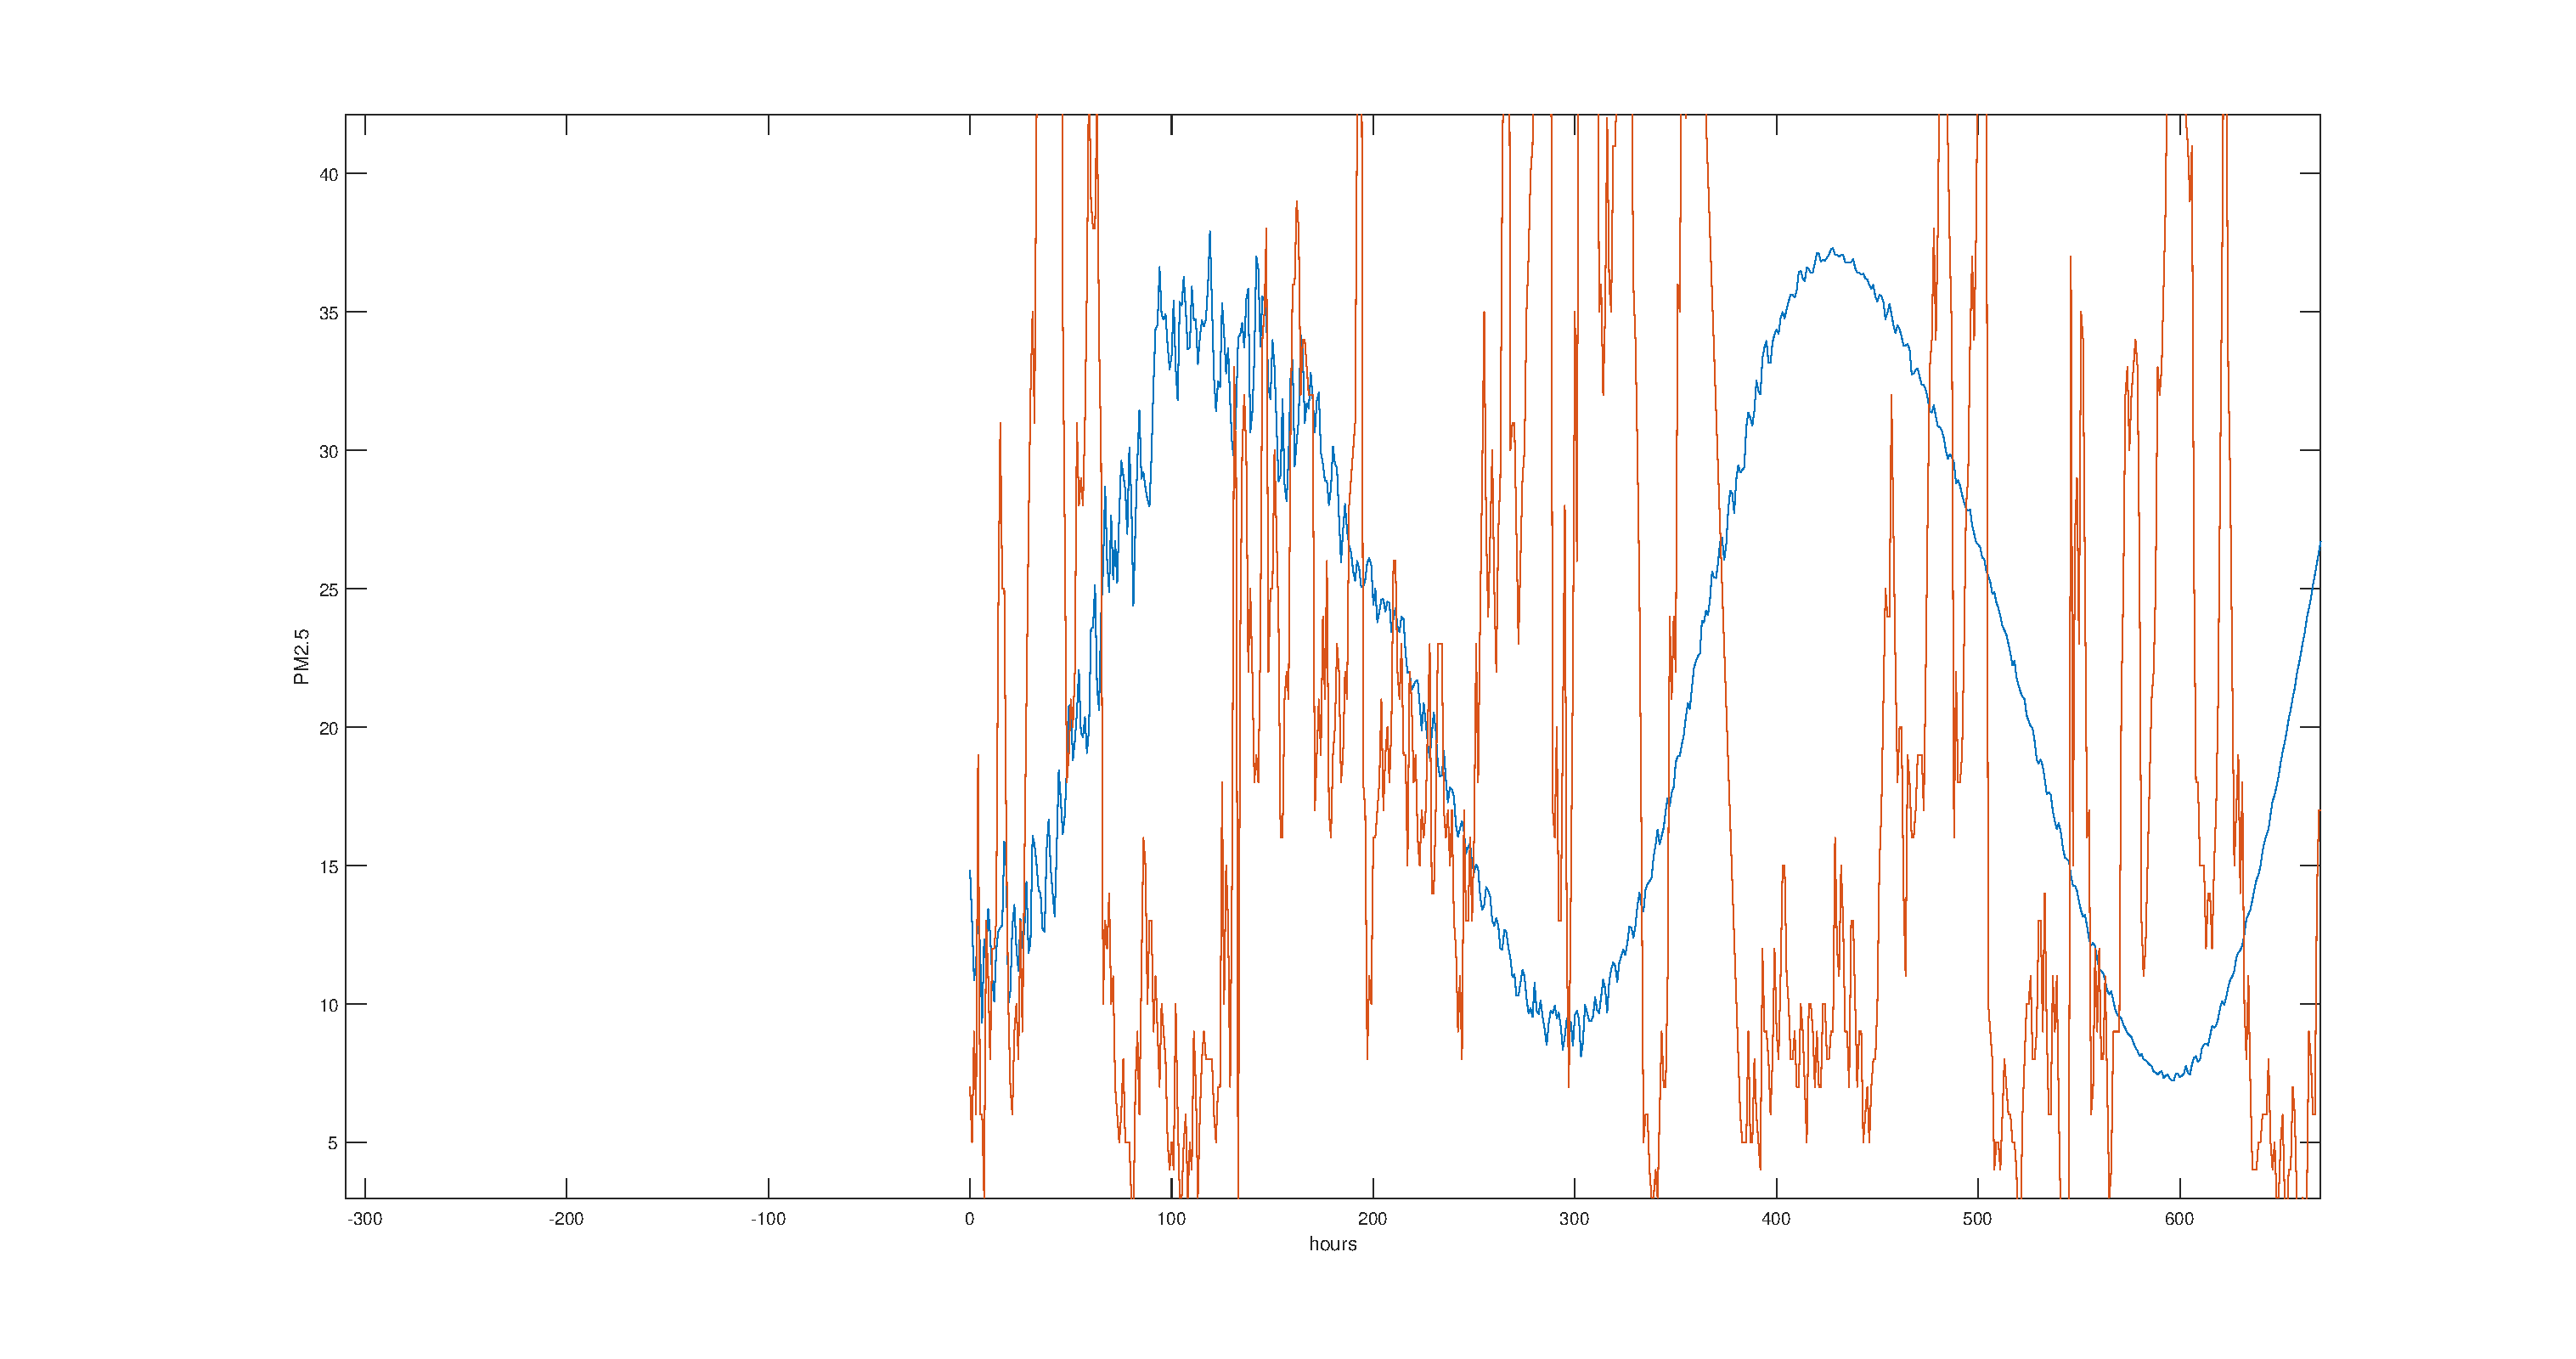
\includegraphics[width=0.9\textwidth]{./picture/untide2.eps} %插入图片,[]中设置图片大小,{}中是图片文件名
    \caption{根均方误差图和损失函数图}
    \label{untide2} 
\end{figure}


表\ref{hours72}只选取了2022年4月12日中午12点后72小时预测的部分数据,并且与2022年4月12日之后72小时的数据进行对比。需要注意的是,本文写作的时间尚未到预测节点后72小时,同时因为此时刻Open-AQ在2022年4月15日10点之前只收集到了2022年4月12日中午12点至2022年4月14日中午12点的数据,共计48个小时的数据,因此能够对比的数据只有40个。完整的对比表格表\ref{allhours72}可以在附录中找到。

\begin{table}[H]
    \centering
    \begin{tabular}{|c|c|clll|}
    \hline
    \multicolumn{1}{|l|}{时间} & \multicolumn{1}{l|}{预测等级} & \multicolumn{4}{l|}{实际等级} \\ \hline
    第1个小时                     & 优                         & \multicolumn{4}{c|}{优}    \\ \hline
    第2个小时                     & 优                         & \multicolumn{4}{c|}{优}    \\ \hline
    ...                     & ...                         & \multicolumn{4}{c|}{...}    \\ \hline
    第71个小时                     & 轻度污染                         & \multicolumn{4}{c|}{尚未发生}    \\ \hline
    第72个小时                    & 轻度污染                         & \multicolumn{4}{c|}{尚未发生}    \\ \hline
    \end{tabular}
    \caption{24实时预测(部分)}
    \label{hours72}
\end{table}

% \subsection{BP神经网络模型设计}
% 首先利用上文的归一化公式进行数据处理,方便进行后面的数据处理,同时保证程序运行时的收敛速度。

% 对数据归一化处理后,初始化BP神经网络时需要根据系统输入、输出序列(X,Y)来确定输入层节点数量、隐含层节点数量、输出层节点数量、目标误差、迭代次数。在对数据特征进行分析后,本系统设定神经网络允许精度 ,最大学习次数 ,隐含层层数为2层,隐含层每层神经元数量为5个,由此建立了如图所示的神经网络结构:
% \begin{figure}[H] %H为当前位置,!htb为忽略美学标准,htbp为浮动图形
%     \centering %图片居中
%     \includegraphics[width=0.7\textwidth]{./picture/network.png} %插入图片,[]中设置图片大小,{}中是图片文件名
%     \caption{神经网络结构} 
% \end{figure}


% 隐含层传输函数采用sigmod函数:
% \begin{equation}
%     f(x)=\frac{1}{1+e^{-x}}
% \end{equation}

% 搭建好神经网络模型后,计算得到计算了将来三个月各项空气指标的变化。
% \begin{figure}[H] %H为当前位置,!htb为忽略美学标准,htbp为浮动图形
%     \centering %图片居中
%     \includegraphics[width=0.7\textwidth]{./picture/sjwl2.png} %插入图片,[]中设置图片大小,{}中是图片文件名
%     \caption{将来三个月空气指标神经网络预测} 
% \end{figure}

% \subsection{灰色预测模型}
% 灰色预测模型进行预测对原始数据进行累加生成,得到近似的指数规律在进行建模。能够利用微分方程充分挖掘系统的本质,精度高;能够将无规律的的原始数据进行生成得到规律性较强的生成序列:
% \begin{equation}
%     x^{(0)}=(x^{(0)}(1),x^{(0)}(2),...,x^{(0)}(n))
% \end{equation}

% 一次累加生成序列:
% \begin{equation}
%     x^{(1)}=(x^{(1)}(1),x^{(1)}(2),...,x^{(1)}(10))=(x^{(0)}(1),x^{(0)}(1)+x^{(0)}(2),...x^{(0)}(1)+...+x^{(0)}(n))
% \end{equation}

% 式中:
% \begin{equation}
%     x^{(1)}(k)=\sum_{i=1}^{k}{x^{(0)}(i),k=1,2,...,n}
% \end{equation}

% $x^{(1)}$的均值生成序列:
% \begin{equation}
%     z^{(1)}=(z^{(1)}(2),z^{(1)}(3),...,z^{(1)}(n))
% \end{equation}

% 式中:
% \begin{equation}
%     z^{(1}(k)=0.5x^{(1)}(k)+0.5x^{(1)}(k-1),k=2,3,...n
% \end{equation}

% 建立灰微分方程:
% \begin{equation}
%     x^{(0)}(k)+az^{(1)}(k)=b,k=2,3,...,n
% \end{equation}

% 相应的白化微分方程为:
% \begin{equation}
%     \frac{dx^{(1)}}{dt}+ax^{(1)}(t)=b
% \end{equation}

% 记
% \begin{equation}
%     u=\left[a,b\right]^T
% \end{equation}

% \begin{equation}
%     Y=[x^{(0)}(2),x^{(0)}(3),...,x^{(0)}(n)^T]
% \end{equation}

% % \begin{equation}
% %     B=\left[\begin{matrix}-z^{(1)}(2)&1\\-z^{(1)}(3)&1\\...&...\\-z^{(1)}(10)&1\\\end{matrix}\right]
% % \end{equation}

% 则由最小二乘法,求得使$J(u)=(Y-Bu)^T(Y-Bu)$达到最小值的u的估计值为

% \begin{equation}
%     \hat{u}=[\hat{a},\hat{b}]T=(BTB)-1BTY
% \end{equation}

% 于是得到方程:
% \begin{equation}
%     \hat{x}(k+1)=(x^{(0)}(1)-\frac{\hat{b}}{\hat{a}})e^{-\hat{a}k}+\frac{\hat{b}}{\hat{a}},k=0,1,...,n 
% \end{equation}

% 灰色预测模型运作时,需要对已知数据进行必要的级比检验,参考数据$x^{(0)}=(x^{(0)}(1),x^{(0)}(2),...,x^0(n))$,计算序列的级比:
% \begin{equation}
%     \lambda(k)=\frac{x^{(0)}(k-1)}{x^{(0}(k)},k=2,3,...n, 
% \end{equation}

% 当计算得到的级比$\lambda(k)$都落在可容覆盖$\theta$内$x^{(0)}$序列 可以作为模型$GM(1,1)$的数据进行预测。

% 将数据导入模型,计算得:
% \begin{figure}[H] %H为当前位置,!htb为忽略美学标准,htbp为浮动图形
%     \centering %图片居中
%     \includegraphics[width=0.7\textwidth]{./picture/hsyc2.png} %插入图片,[]中设置图片大小,{}中是图片文件名
%     \caption{未来三个月指标灰色预测} 
% \end{figure}s

% 未来三个月$PM_{2.5}$、$PM_{10}$及AQI的值分别在90到100,70到80,50到60左右。

\newpage
\section{北京市朝阳区空气污染治理状况及对策}
北京历史上曾在北京和环北京区域的相邻省份采取过极端的减排措施,但是在"APEC"会议时期$PM_{2.5}$的浓度依然高达51.5微克/立方米$^{[4]}$。大气污染具有时间关系和周期关系,应当利用周期规律进行合理的减排手段,实现逐年提高空气质量。

\begin{figure}[H] %H为当前位置,!htb为忽略美学标准,htbp为浮动图形
    \centering %图片居中
    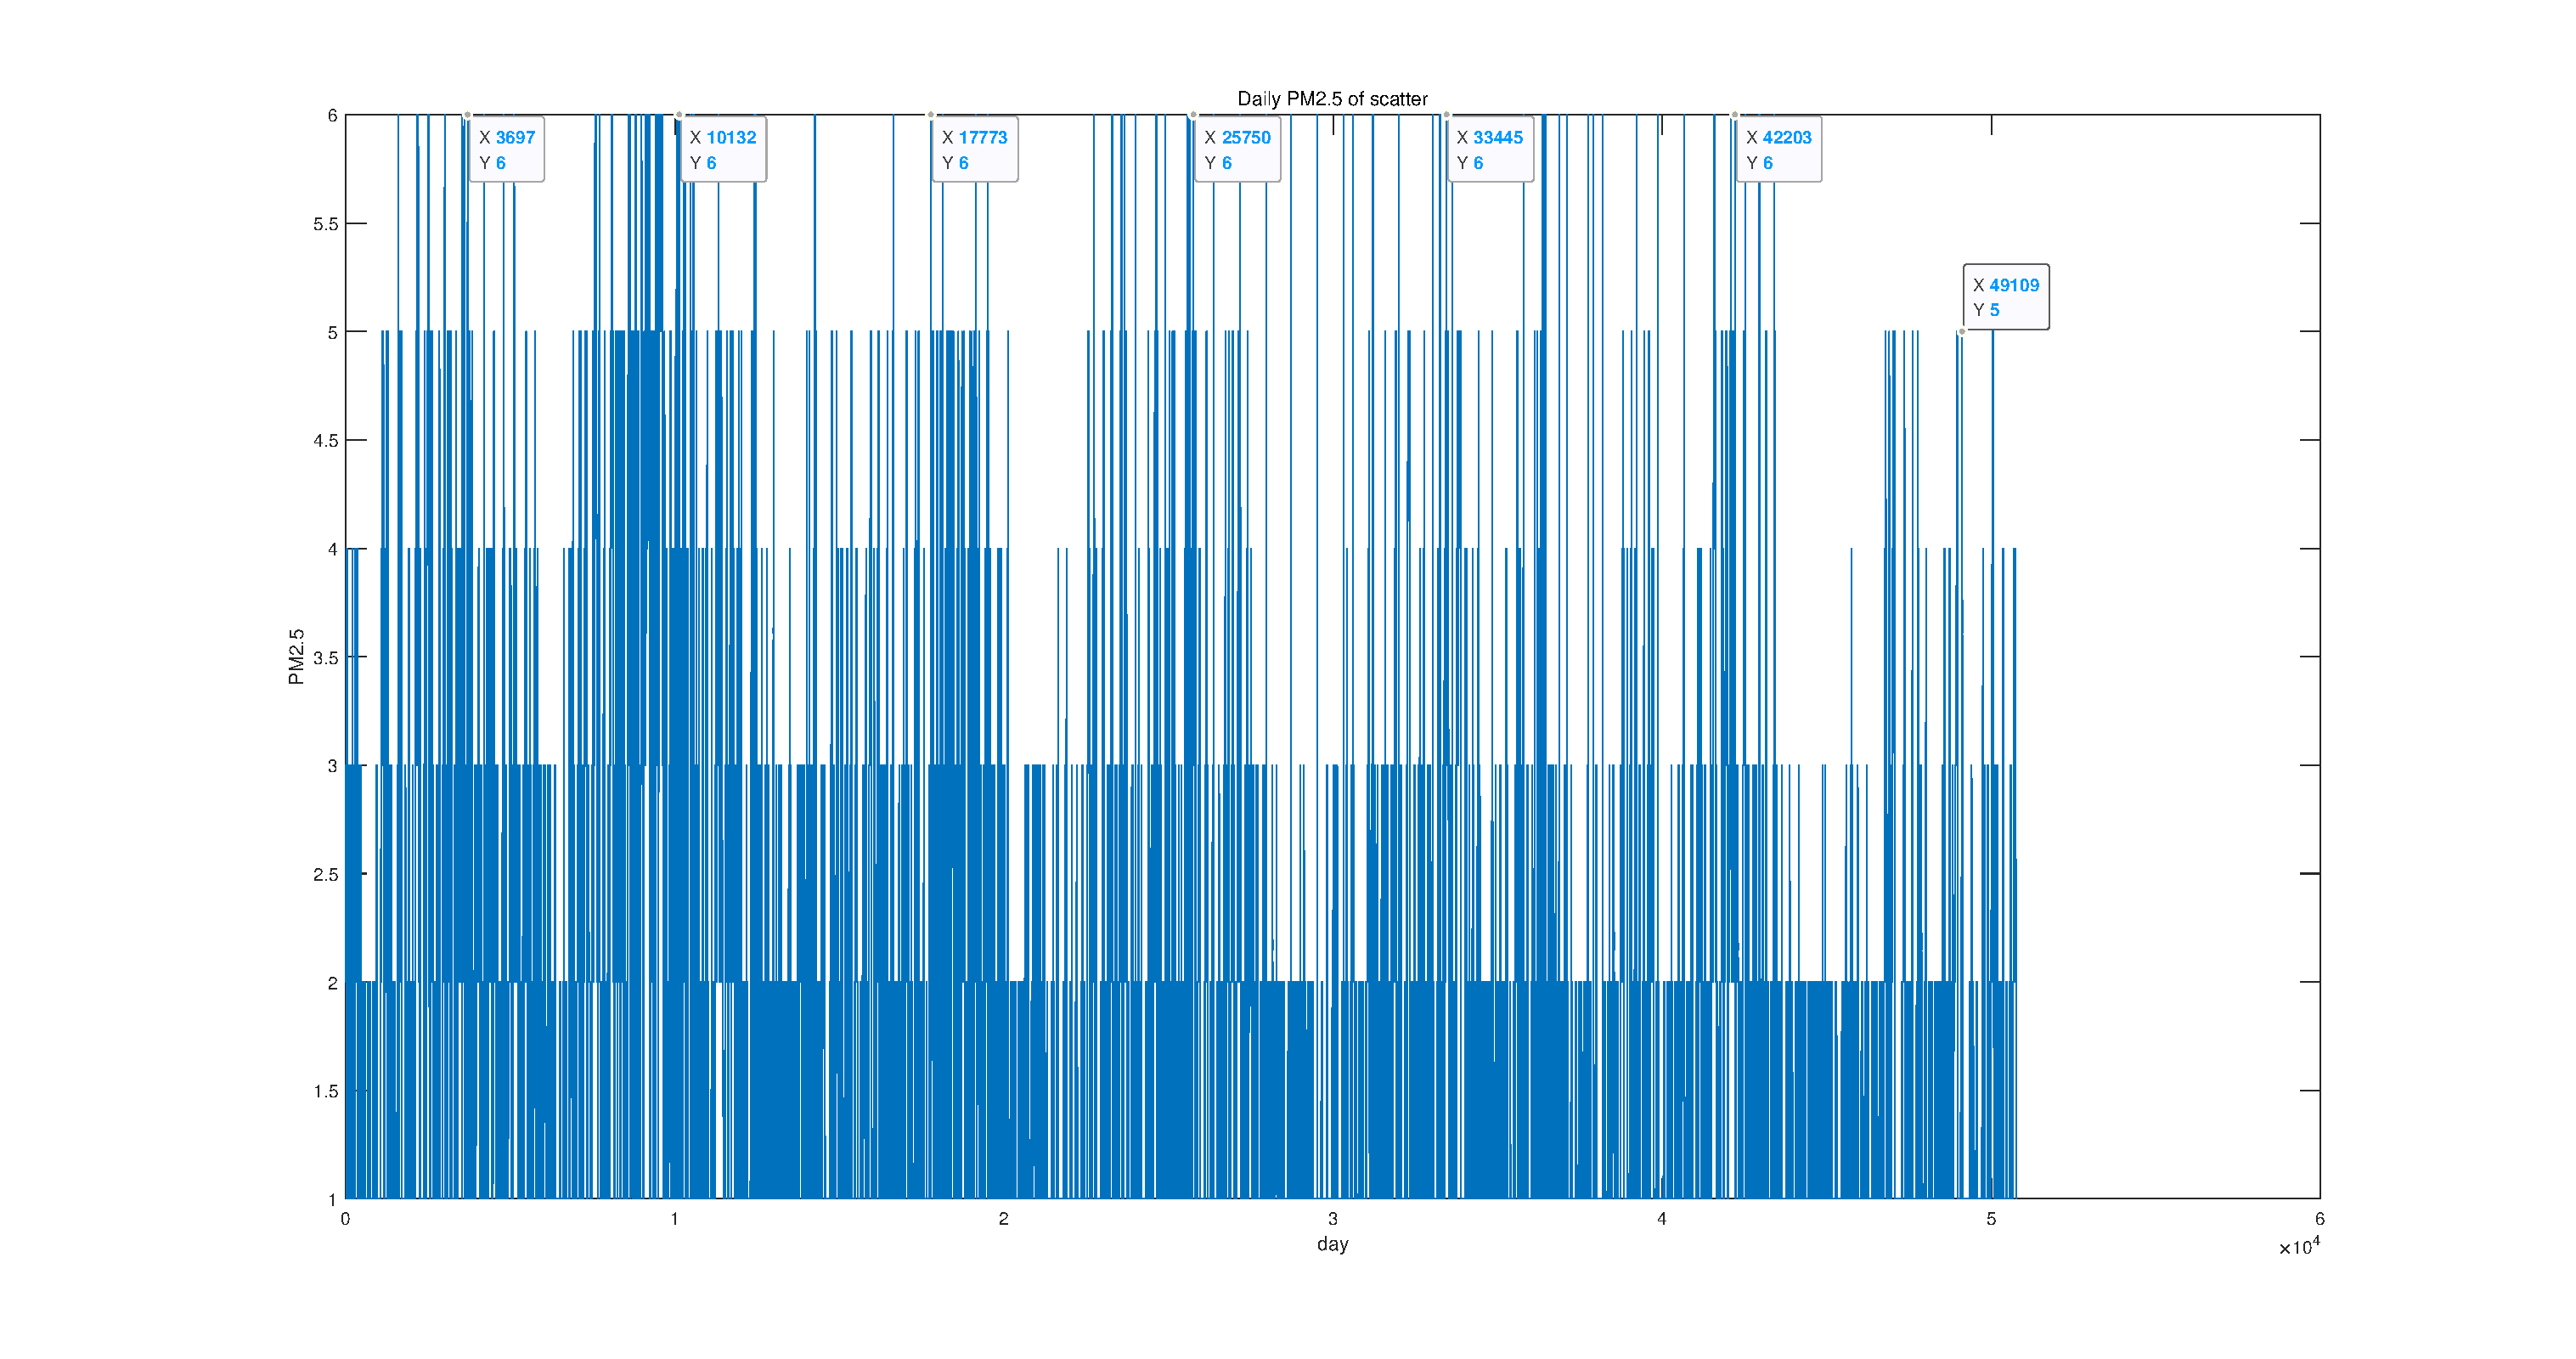
\includegraphics[width=1\textwidth]{./picture/TimeRule.eps} %插入图片,[]中设置图片大小,{}中是图片文件名
    \caption{$PM_{2.5}$高峰周期} 
\end{figure}
根据$PM_{2.5}$高峰周期图可以得出,$PM_{2.5}$的周期基本上是以一年为一个周期,在每年从入冬到开春是空气质量最差的时期,由于供暖和更多的私家车上路,造成空气污染更为严重。应对此种现象,可以考虑采用清洁能源取暖,减少燃煤取暖;同时在冬季来临之前的三个月内提前适当限行车辆,减少尾气排放。为了遏制北京空气质量的恶化,后续应重点控制电力、热力生产企业、黑色金属、有色金属行业的废气排放量。

其中电力行业产生的废气多的原因主要是由于我国的新能源装机容量不足,截至2020年底,全国电源总装机容量超过22亿千瓦,火电水电仍为第一第二大电源,分别占比57\%,17\%。当前电力行业二氧化碳排放约占中国能源活动二氧化碳排放的40\%。2020年全社会用电量为7.5万亿千瓦时,十三五期间全社会用电量年均增速为5.7\%。利用新能源代替传统发电仍需继续研究,逐步推进。拉闸限电势在必行。对于相关部门而言,应加大重点行业排放的监督力度,引导企业做好生产后的废气净化处理,加大投入。减少火力发电,引进新能源发电技术迫在眉睫。
\begin{figure}[H]
    \centering
\begin{tikzpicture}[]
    \pie[text=legend]{0.5438/黑色金属矿采选业,0.7795/有色金属矿采选业,1.0957/农副产品加工业,0.02/造纸及纸制品业,17.9507/石油加工炼焦及核燃料加工业,2.4036/化学原料及化学制品制造业,16.732/非金属矿物制品业,5.3756/黑色金属冶炼及压延加工业,3.5854/有色金属冶炼及压延加工业,32.6881/电力、热力的生产和供应业,18.6456/其他行业}
\end{tikzpicture}
\caption{各行用电占比}
\end{figure}

\newpage
\section{研究结论总结}
本文以Matlab2019、SPSSPro等软件作为编程语言和分析工具。通过使用基于TOPSIS的环境评价模型,可以分析一个地区历年的环境发展变化,也可以分析多个地区同一年的环境发展情况,为环境政策的有效性提供了客观的参考的指标。本文以塞罕坝三十余年的数据进行分析,得出了每个时期塞罕坝的环境发展质量的评价水平。同时利用该模型对全国各大省、直辖市(除台湾省以及香港特别行政区和澳门特别行动区)进行了分析和排名,并绘制了全国环境质量发展热力图,得出了我国目前环北京地区,华北平原以及黄河中下游省份环境质量较差,我国越往南的地区环境质量越好的结论。

其次使用北京市朝阳区从2015年7月7日中午12点到2022年4月12日中午12点每个小时的$PM_{2.5}$的含量训练了两个LSTM神经网络模型,分别用于实时预测和72小时预测北京市朝阳区今后$PM_{2.5}$的含量,并分析了北京市朝阳区$PM_{2.5}$出现的周期现象,提出了针对$PM_{2.5}$周期治理的政策建议。

% \begin{figure}[H] %H为当前位置,!htb为忽略美学标准,htbp为浮动图形
%     \centering %图片居中
%     \includegraphics[width=0.9\textwidth]{./picture/geshenglsf.png} %插入图片,[]中设置图片大小,{}中是图片文件名
%     \caption{近四次全国森林覆盖率} 
% \end{figure}

% \begin{figure}[H] %H为当前位置,!htb为忽略美学标准,htbp为浮动图形
%     \centering %图片居中
%     \includegraphics[width=1\textwidth]{./picture/newrate.png} %插入图片,[]中设置图片大小,{}中是图片文件名
%     \caption{近四次全国森林覆盖率变化率} 
% \end{figure}

近年“绿水青山就是金山银山”政策以及“碳达峰、碳中和”目标的提出,越来越多的学者、专家将目光投入环境评价和预测中去。随着计算机技术的发展,待更多的优秀的评价预测算法的出现,可把大气环境评价预测推进到一个更高的水平。

\newpage
\section{参考文献}
[1]李丽. 基于数据挖掘的城市环境空气质量决策支持系统设计与实现[D].山东师范大学,2006.

[2]马媛媛,孙世群.模糊综合评价在合肥市大气环境评价中的应用[J].环境科学与管理,2012,37(05):188-191.

[3]金文彪,姚永杰,金哲植.基于主成分分析的大气环境预测研究[J].科教导刊(中旬刊),2016(32):148-150.DOI:10.16400/j.cnki.kjdkz.2016.11.071.

[4]北京大学统计科学中心,北京大学光华管理学院.北京城区2010-2014年$PM_{2.5}$污染状况研究[J].2015.3.

[5]Endah Kristiani, Hao Lin, Jwu-Rong Lin, Yen-Hsun Chuang, Chin-Yin Huang and Chao-Tung Yang.5Short-Term Prediction of $PM_{2.5}$ Using LSTM Deep Learning Methods[J].Sustainability 2022, 14, 2068.

[6]袁冲.基于熵权法的江苏省各市经济高质量发展评价分析[J].商业经济,2022(04):19-20+42.DOI:10.19905/j.cnki.syjj1982.2022.04.061.

[7]徐政华,曹延明.基于熵权TOPSIS模型的长春市水资源承载力评价[J/OL].安全与环境学报:1-10[2022-03-27].DOI:10.13637/j.issn.1009-6094.2021.1448


\appendix
\section{附录}
\subsection{完整的预测表格}
\subsubsection{24小时$PM_{2.5}$实时预测表格}

\begin{table}[H]
    \centering
    \begin{tabular}{|l|l|l|}
        \hline
        时间    & 预测等级 & 实际等级 \\ \hline
        第1小时  & 优    & 优    \\ \hline
        第2小时  & 优    & 优    \\ \hline
        第3小时  & 优    & 优    \\ \hline
        第4小时  & 优    & 优    \\ \hline
        第5小时  & 优    & 优    \\ \hline
        第6小时  & 优    & 优    \\ \hline
        第7小时  & 优    & 优    \\ \hline
        第8小时  & 优    & 优    \\ \hline
        第9小时  & 优    & 优    \\ \hline
        第10小时 & 优    & 优    \\ \hline
        第11小时 & 优    & 优    \\ \hline
        第12小时 & 优    & 优    \\ \hline
        第13小时 & 优    & 优    \\ \hline
        第14小时 & 优    & 优    \\ \hline
        第15小时 & 优    & 优    \\ \hline
        第16小时 & 优    & 优    \\ \hline
        第17小时 & 优    & 优    \\ \hline
        第18小时 & 优    & 优    \\ \hline
        第19小时 & 优    & 优    \\ \hline
        第20小时 & 优    & 优    \\ \hline
        第21小时 & 优    & 优    \\ \hline
        第22小时 & 优    & 优    \\ \hline
        第23小时 & 优    & 优    \\ \hline
        第24小时 & 优    & 优    \\ \hline
        \end{tabular}
    \caption{24实时预测}
    \label{allhours24}
\end{table}


\subsubsection{72小时$PM_{2.5}$预测表格}
\begin{table}[H]
    \centering
    \begin{tabular}{|l|l|l|l|l|l|}
        \hline
        时间    & 预测等级 & 实际等级 & 时间    & 预测等级 & 实际等级 \\ \hline
        第1小时  & 优    & 优    & 第37小时 & 良    & 优    \\ \hline
        第2小时  & 优    & 优    & 第38小时 & 良    & 良    \\ \hline
        第3小时  & 优    & 优    & 第39小时 & 良    & 良    \\ \hline
        第4小时  & 优    & 优    & 第40小时 & 良    & 优    \\ \hline
        第5小时  & 优    & 优    & 第41小时 & 良    & 优    \\ \hline
        第6小时  & 优    & 优    & 第42小时 & 良    & 优    \\ \hline
        第7小时  & 优    & 优    & 第43小时 & 良    & 优    \\ \hline
        第8小时  & 优    & 优    & 第44小时 & 良    & 优    \\ \hline
        第9小时  & 优    & 优    & 第45小时 & 良    & 优    \\ \hline
        第10小时 & 优    & 优    & 第46小时 & 良    & 优    \\ \hline
        第11小时 & 优    & 优    & 第47小时 & 良    & 优    \\ \hline
        第12小时 & 优    & 优    & 第48小时 & 良    & 优    \\ \hline
        第13小时 & 优    & 优    & 第49小时 & 良    & 暂无数据 \\ \hline
        第14小时 & 优    & 优    & 第50小时 & 良    & 暂无数据 \\ \hline
        第15小时 & 优    & 优    & 第51小时 & 良    & 暂无数据 \\ \hline
        第16小时 & 优    & 优    & 第52小时 & 良    & 暂无数据 \\ \hline
        第17小时 & 优    & 优    & 第53小时 & 良    & 暂无数据 \\ \hline
        第18小时 & 优    & 优    & 第54小时 & 良    & 暂无数据 \\ \hline
        第19小时 & 优    & 优    & 第55小时 & 良    & 暂无数据 \\ \hline
        第20小时 & 优    & 优    & 第56小时 & 良    & 暂无数据 \\ \hline
        第21小时 & 优    & 优    & 第57小时 & 良    & 暂无数据 \\ \hline
        第22小时 & 优    & 优    & 第58小时 & 良    & 暂无数据 \\ \hline
        第23小时 & 优    & 优    & 第59小时 & 良    & 暂无数据 \\ \hline
        第24小时 & 优    & 优    & 第60小时 & 良    & 暂无数据 \\ \hline
        第25小时 & 优    & 优    & 第61小时 & 良    & 暂无数据 \\ \hline
        第26小时 & 优    & 优    & 第62小时 & 良    & 暂无数据 \\ \hline
        第27小时 & 优    & 优    & 第63小时 & 良    & 暂无数据 \\ \hline
        第28小时 & 优    & 优    & 第64小时 & 轻度污染 & 暂无数据 \\ \hline
        第29小时 & 优    & 优    & 第65小时 & 轻度污染 & 暂无数据 \\ \hline
        第30小时 & 优    & 优    & 第66小时 & 轻度污染 & 暂无数据 \\ \hline
        第31小时 & 良    & 优    & 第67小时 & 轻度污染 & 暂无数据 \\ \hline
        第32小时 & 良    & 优    & 第68小时 & 轻度污染 & 暂无数据 \\ \hline
        第33小时 & 良    & 优    & 第69小时 & 轻度污染 & 暂无数据 \\ \hline
        第34小时 & 良    & 优    & 第70小时 & 轻度污染 & 暂无数据 \\ \hline
        第35小时 & 良    & 优    & 第71小时 & 轻度污染 & 暂无数据 \\ \hline
        第36小时 & 良    & 良    & 第72小时 & 轻度污染 & 暂无数据 \\ \hline
        \end{tabular}
    \caption{24实时预测}
    \label{allhours72}
\end{table}

\subsection{相关代码}
\subsubsection{$TOSIS$综合评价代码}
\begin{figure}[H] %H为当前位置,!htb为忽略美学标准,htbp为浮动图形
    \centering %图片居中
    \includegraphics[width=1.2\textwidth]{./code/ESS.pdf} %插入图片,[]中设置图片大小,{}中是图片文件名
\end{figure}

\begin{figure}[H] %H为当前位置,!htb为忽略美学标准,htbp为浮动图形
    \centering %图片居中
    \includegraphics[width=1.2\textwidth,page=1]{./code/CA.pdf} %插入图片,[]中设置图片大小,{}中是图片文件名
\end{figure}

\begin{figure}[H] %H为当前位置,!htb为忽略美学标准,htbp为浮动图形
    \centering %图片居中
    \includegraphics[width=1.2\textwidth,page=2]{./code/CA.pdf} %插入图片,[]中设置图片大小,{}中是图片文件名
\end{figure}

\begin{figure}[H] %H为当前位置,!htb为忽略美学标准,htbp为浮动图形
    \centering %图片居中
    \includegraphics[width=1.2\textwidth,page=3]{./code/CA.pdf} %插入图片,[]中设置图片大小,{}中是图片文件名
\end{figure}

\begin{figure}[H] %H为当前位置,!htb为忽略美学标准,htbp为浮动图形
    \centering %图片居中
    \includegraphics[width=1.2\textwidth,page=4]{./code/CA.pdf} %插入图片,[]中设置图片大小,{}中是图片文件名
\end{figure}

\subsubsection{热力图生成代码}
\begin{figure}[H] %H为当前位置,!htb为忽略美学标准,htbp为浮动图形
    \centering %图片居中
    \includegraphics[width=1.2\textwidth]{./code/ChinaMap.pdf} %插入图片,[]中设置图片大小,{}中是图片文件名
\end{figure}

\subsubsection{$PM_{2.5}$实时预测LSTM神经网络代码}
\begin{figure}[H] %H为当前位置,!htb为忽略美学标准,htbp为浮动图形
    \centering %图片居中
    \includegraphics[width=1.2\textwidth,page=1]{./code/BeijingNet1.pdf} %插入图片,[]中设置图片大小,{}中是图片文件名
\end{figure}
\begin{figure}[H] %H为当前位置,!htb为忽略美学标准,htbp为浮动图形
    \centering %图片居中
    \includegraphics[width=1.2\textwidth,page=2]{./code/BeijingNet1.pdf} %插入图片,[]中设置图片大小,{}中是图片文件名
\end{figure}
\begin{figure}[H] %H为当前位置,!htb为忽略美学标准,htbp为浮动图形
    \centering %图片居中
    \includegraphics[width=1.2\textwidth,page=3]{./code/BeijingNet1.pdf} %插入图片,[]中设置图片大小,{}中是图片文件名
\end{figure}
\begin{figure}[H] %H为当前位置,!htb为忽略美学标准,htbp为浮动图形
    \centering %图片居中
    \includegraphics[width=1.2\textwidth,page=4]{./code/BeijingNet1.pdf} %插入图片,[]中设置图片大小,{}中是图片文件名
\end{figure}
\begin{figure}[H] %H为当前位置,!htb为忽略美学标准,htbp为浮动图形
    \centering %图片居中
    \includegraphics[width=1.2\textwidth,page=5]{./code/BeijingNet1.pdf} %插入图片,[]中设置图片大小,{}中是图片文件名
\end{figure}
\begin{figure}[H] %H为当前位置,!htb为忽略美学标准,htbp为浮动图形
    \centering %图片居中
    \includegraphics[width=1.2\textwidth,page=6]{./code/BeijingNet1.pdf} %插入图片,[]中设置图片大小,{}中是图片文件名
\end{figure}
\begin{figure}[H] %H为当前位置,!htb为忽略美学标准,htbp为浮动图形
    \centering %图片居中
    \includegraphics[width=1.2\textwidth,page=7]{./code/BeijingNet1.pdf} %插入图片,[]中设置图片大小,{}中是图片文件名
\end{figure}
\begin{figure}[H] %H为当前位置,!htb为忽略美学标准,htbp为浮动图形
    \centering %图片居中
    \includegraphics[width=1.2\textwidth,page=8]{./code/BeijingNet1.pdf} %插入图片,[]中设置图片大小,{}中是图片文件名
\end{figure}
\begin{figure}[H] %H为当前位置,!htb为忽略美学标准,htbp为浮动图形
    \centering %图片居中
    \includegraphics[width=1.2\textwidth,page=9]{./code/BeijingNet1.pdf} %插入图片,[]中设置图片大小,{}中是图片文件名
\end{figure}
\begin{figure}[H] %H为当前位置,!htb为忽略美学标准,htbp为浮动图形
    \centering %图片居中
    \includegraphics[width=1.2\textwidth,page=10]{./code/BeijingNet1.pdf} %插入图片,[]中设置图片大小,{}中是图片文件名
\end{figure}
\begin{figure}[H] %H为当前位置,!htb为忽略美学标准,htbp为浮动图形
    \centering %图片居中
    \includegraphics[width=1.2\textwidth,page=11]{./code/BeijingNet1.pdf} %插入图片,[]中设置图片大小,{}中是图片文件名
\end{figure}

\begin{figure}[H] %H为当前位置,!htb为忽略美学标准,htbp为浮动图形
    \centering %图片居中
    \includegraphics[width=1.2\textwidth,page=12]{./code/BeijingNet1.pdf} %插入图片,[]中设置图片大小,{}中是图片文件名
\end{figure}

\subsubsection{$PM_{2.5}$72小时预测LSTM神经网络代码}

\begin{figure}[H] %H为当前位置,!htb为忽略美学标准,htbp为浮动图形
    \centering %图片居中
    \includegraphics[width=1.2\textwidth,page=1]{./code/BeijingNet2.pdf} %插入图片,[]中设置图片大小,{}中是图片文件名
\end{figure}

\begin{figure}[H] %H为当前位置,!htb为忽略美学标准,htbp为浮动图形
    \centering %图片居中
    \includegraphics[width=1.2\textwidth,page=2]{./code/BeijingNet2.pdf} %插入图片,[]中设置图片大小,{}中是图片文件名
\end{figure}

\begin{figure}[H] %H为当前位置,!htb为忽略美学标准,htbp为浮动图形
    \centering %图片居中
    \includegraphics[width=1.2\textwidth,page=3]{./code/BeijingNet2.pdf} %插入图片,[]中设置图片大小,{}中是图片文件名
\end{figure}

\begin{figure}[H] %H为当前位置,!htb为忽略美学标准,htbp为浮动图形
    \centering %图片居中
    \includegraphics[width=1.2\textwidth,page=4]{./code/BeijingNet2.pdf} %插入图片,[]中设置图片大小,{}中是图片文件名
\end{figure}

\begin{figure}[H] %H为当前位置,!htb为忽略美学标准,htbp为浮动图形
    \centering %图片居中
    \includegraphics[width=1.2\textwidth,page=5]{./code/BeijingNet2.pdf} %插入图片,[]中设置图片大小,{}中是图片文件名
\end{figure}

\begin{figure}[H] %H为当前位置,!htb为忽略美学标准,htbp为浮动图形
    \centering %图片居中
    \includegraphics[width=1.2\textwidth,page=6]{./code/BeijingNet2.pdf} %插入图片,[]中设置图片大小,{}中是图片文件名
\end{figure}

\begin{figure}[H] %H为当前位置,!htb为忽略美学标准,htbp为浮动图形
    \centering %图片居中
    \includegraphics[width=1.2\textwidth,page=7]{./code/BeijingNet2.pdf} %插入图片,[]中设置图片大小,{}中是图片文件名
\end{figure}

\begin{figure}[H] %H为当前位置,!htb为忽略美学标准,htbp为浮动图形
    \centering %图片居中
    \includegraphics[width=1.2\textwidth,page=8]{./code/BeijingNet2.pdf} %插入图片,[]中设置图片大小,{}中是图片文件名
\end{figure}

\begin{figure}[H] %H为当前位置,!htb为忽略美学标准,htbp为浮动图形
    \centering %图片居中
    \includegraphics[width=1.2\textwidth,page=9]{./code/BeijingNet2.pdf} %插入图片,[]中设置图片大小,{}中是图片文件名
\end{figure}

\begin{figure}[H] %H为当前位置,!htb为忽略美学标准,htbp为浮动图形
    \centering %图片居中
    \includegraphics[width=1.2\textwidth,page=10]{./code/BeijingNet2.pdf} %插入图片,[]中设置图片大小,{}中是图片文件名
\end{figure}

\begin{figure}[H] %H为当前位置,!htb为忽略美学标准,htbp为浮动图形
    \centering %图片居中
    \includegraphics[width=1.2\textwidth,page=11]{./code/BeijingNet2.pdf} %插入图片,[]中设置图片大小,{}中是图片文件名
\end{figure}

\end{document}